\documentclass[12pt, titlepage]{article}


\usepackage{lscape}
\usepackage{amsmath, mathtools}
\usepackage{amsfonts}
\usepackage{amssymb}
\usepackage{graphicx}
\usepackage{colortbl}
\usepackage{xr}
\usepackage{hyperref}
\usepackage{longtable}
\usepackage{xfrac}
\usepackage{tabularx}
\usepackage{float}
\usepackage{siunitx}
\usepackage{booktabs}
\usepackage{caption}
\usepackage{pdflscape}
\usepackage{afterpage}
\usepackage{multirow}
\usepackage{listings}

\hypersetup{
    colorlinks,
    citecolor=black,
    filecolor=black,
    linkcolor=red,
    urlcolor=blue
}

\newcounter{reqnum} %Requirement Number
\newcommand{\rthereqnum}{P\thereqnum}
\newcommand{\rref}[1]{R\ref{#1}}

\usepackage[round]{natbib}
\usepackage{longtable}
\usepackage{lscape}

\externaldocument[CA-]{../../Commonality-Analysis/CA}

%% Comments

\usepackage{color}

\newif\ifcomments\commentstrue

\ifcomments
\newcommand{\authornote}[3]{\textcolor{#1}{[#3 ---#2]}}
\newcommand{\todo}[1]{\textcolor{red}{[TODO: #1]}}
\else
\newcommand{\authornote}[3]{}
\newcommand{\todo}[1]{}
\fi

\newcommand{\wss}[1]{\authornote{blue}{SS}{#1}} 
\newcommand{\plt}[1]{\authornote{magenta}{TPLT}{#1}} %For explanation of the template
\newcommand{\an}[1]{\authornote{cyan}{Author}{#1}}

%% Common Parts

\newcommand{\progname}{ProgName} % PUT YOUR PROGRAM NAME HERE %Every program
                                % should have a name



\newcommand{\famname}{Lights, Camera, Models!}

\begin{document}

\title{Lights, Camera, Models!: System Verification and Validation Plan for 
Family of Lighting Models} 
\author{Sasha Soraine}
\date{\today}
	
\maketitle

\pagenumbering{roman}

\section{Revision History}

\begin{tabularx}{\textwidth}{p{3cm}p{2cm}X}
\toprule {\bf Date} & {\bf Version} & {\bf Notes}\\
\midrule
October 17, 2019 & 0.1 & Original Draft.\\
November 4, 2019 & 1.0 & Version 1 - Submitted for class.\\
December 18, 2019 & 2.0 & Version 2 \\
\bottomrule
\end{tabularx}

\newpage

\tableofcontents

\listoftables

\listoffigures

\newpage

\section{Symbols, Abbreviations and Acronyms}
\subsection{Table of Units}

Throughout this document SI (Syst\`{e}me International d'Unit\'{e}s) is employed
as the unit system.  In addition to the basic units, several derived units are
used as described below.  For each unit, the symbol is given followed by a
description of the unit and the SI name.
~\newline

\renewcommand{\arraystretch}{1.2}
%\begin{table}[ht]
\noindent \begin{tabular}{l l l} 
	\toprule		
	\textbf{symbol} & \textbf{unit} & \textbf{SI}\\
	\midrule 
	\si{\radian} & angle & radian\\
	\si{cd} & luminous intensity & candela\\	
	\bottomrule
\end{tabular}
%	\caption{Provide a caption}
%\end{table}

\subsection{Table of Symbols}

The table that follows summarizes the symbols used in this document along with
their units.  The choice of symbols was made to be consistent with the physics
and calculus notation. The symbols are listed in alphabetical order.

\renewcommand{\arraystretch}{1.2}
%\noindent \begin{tabularx}{1.0\textwidth}{l l X}
\noindent \begin{longtable*}{l l p{12cm}} \toprule
	\textbf{symbol} & \textbf{unit} & \textbf{description}\\
	\midrule 
	$\mathbb{R}$ & --- & Set of Real numbers.\\
	$\mathbb{Z}$ & --- & Set of Integers.\\
	$\mathbb{Z_{+}}$ & --- & Set of Positive Integers.\\
	$\theta$ & \si[per-mode=symbol] {\radian} & Angle between the viewer and the
	reflected ray.	\\
	$p$ & --- & Point in space or on a surface.
	\\
	$p_{0}$ & --- & Point of origin.
	\\
	$v$ & --- & Position of viewer represented as a 3D point in space.
	\\
	$L_{i}$ & --- & Vector form of incident ray.
	\\
	$L_{r}$ & --- & Vector form of reflected ray.
	\\
	$V$ & --- & Vector from point to the viewer.
	\\
	$n$ & --- & Vector form of surface normal.
	\\
	$N$ & --- & Unit vector of surface normal, $n$.
	\\
	$H$ & --- & Unit vector halfway between the incident ray, $L_{i}$, and
	the viewer vector, $V$.
	\\
	$I_{a}$ & cd & Ambient luminous intensity.
	\\
	$k_{a}$ & -- & Coefficient of Ambient Reflection.
	\\
	$I_{d}$ & cd & Diffuse luminous intensity.
	\\
	$k_{d}$ & -- & Coefficient of Diffuse Reflection.
	\\
	$I_{s}$ & cd & Specular luminous intensity.
	\\
	$k_{s}$ & -- & Coefficient of Specular Reflection.
	\\
	$\alpha$ & -- & Shininess Coefficient.
	\\
	$I_{T}$ & cd & Total luminous intensity.
	\\
	\bottomrule
\end{longtable*}

\subsection{Abbreviations and Acronyms}

\renewcommand{\arraystretch}{1.2}
\begin{tabular}{l l} 
	\toprule		
	\textbf{symbol} & \textbf{description}\\
	\midrule 
	GS & Goal Statement\\
	LC & Likely Change\\
	R & Requirement\\
	CA & Commonality Analysis \\
	LM & Lighting Model\\
	T & Theoretical Model\\
	3D & Three Dimensional \\
	API & Application Programming Interface \\
	\bottomrule
\end{tabular}\\

\newpage

\pagenumbering{arabic}

This document outlines a system validation and verification plan for Lights, 
Camera, Models!, an implementation of a family of lighting models, based on the 
Commonality Analysis (CA) for a family of lighting models 
\url{https://github.com/sorainsm/library-of-lighting-models/tree/master/Commonality-Analysis}.
\wss{I suggest a citation to your  commonality analysis, and/or a link to the 
github location for the document.}
First it will cover general information about the system, including the
particular design qualities the system should emphasize and any relevant
documentation. Next it will outline the verification plans for the commonality
analysis/requirements, system design, and implementation. It will then outline
the software validation plan.  Finally it will outline a series of
representative test cases that are meant to test the functional and
non-functional requirements, along with a traceability matrix mapping the test
cases to particular requirements.

\section{General Information}

\subsection{Summary}
This software implements a sub-family of lighting models. The larger family and 
problem analysis is found in CA. The software discussed in the CA has two 
purposes: education through a usable learning software, and graphics creation 
through the open-source lighting and shader code. For the purposes of  this 
course we focus on creating the learning software, as it will use the open 
source code that fits the graphics creation context.

The \famname application will present the user with a simple scene of a sphere 
in a room with a spot light. The user can modify the material properties of the 
sphere, and the position and type of the light source. \famname will re-render 
the scene in real time to account for these modifications. The calculations 
used to find how to render this are explained in the CA. 

\subsection{Objectives}
The goal of this testing is to:

\begin{itemize}
	\item Demonstrate adequate usability of the system,
	\item Evaluate the productivity of the open source library system.
\end{itemize}

Demonstrating usability of the system means that we look to see how ``easy'' 
the learning context is to use. This involves evaluating the graphical user 
interface that mediates the changes to the scene.

Evaluating productivity of the open source library system means examining how 
quickly we can build a scene using the lighting model library. This testing, 
while aimed as a system level test, will be conducted after the completion of 
this course.

%\wss{State what is intended to be accomplished.  The objective will be around
%  the qualities that are most important for your project.  You might have
%  something like: ``build confidence in the software correctness,''
%  ``demonstrate adequate usability.'' etc.  You won't list all of the 
%qualities,
%  just those that are most important.}

\pagebreak
\subsection{Relevant Documentation}
This section outlines other documentation that is relevant for understanding 
this document.
\begin{table}[h]
	\begin{tabular}{|p{3.5cm}|p{3cm}|p{8cm}|}
		\hline
	\textbf{Document Name} & \textbf{Document Type} & \textbf{Document Purpose} 
	 \\
		\hline
		Commonality Analysis of a Family of Lighting Models& Commonality 
		Analysis & Problem domain description, and scoping to a reasonable 
		implementation size through assumptions and requirements. \\ 
		\hline
	\end{tabular}
\end{table}
%\wss{Reference relevant documentation.  This will definitely include your SRS}

\section{Plan}
This section outlines the verification and validation plans, including any 
techniques or data sets being used in the testing process. It also outlines the 
members of the verification and validations team.
	
\subsection{Verification and Validation Team}
This section lists the members of the verification and validation team. These 
are individuals who contribute to the verification and validation of the system 
and software design. Individuals listed here have specific roles denoting the 
amount of involvement they will be having in the verification and validation 
process. Primary roles are actively working on it; secondary roles view the 
system when major submissions are made; tertiary roles are asked to contribute 
if able, but are under no obligation to participate.

The verification and validation team includes:

\begin{table}[h]
	\begin{tabular}{|l|l|p{8cm}|}
		\hline
		\textbf{Name} & \textbf{Role} & \textbf{Goal} \\
		\hline
		Sasha Soraine & Primary Reviewer& Ensure the verification and 
		validation 
		process runs smoothly.\\
		Peter Michalski & Secondary Reviewer& Ensure the logical consistency of 
		system 
		design and requirements in accordance with feedback role as expert 
		reviewer. \\
		Dr. Spencer Smith & Secondary Reviewer& Ensure reasonable coverage of 
		design 
		considerations and requirements as part of marking these documents. \\
		CAS 741 Students & Tertiary Reviewers& Ensure general consistency in 
		design and 
		requirements coverage in accordance with feedback role as secondary 
		reviewers.\\
		\hline
	\end{tabular}
\end{table}

\wss{If you use the booktabs package, your tables will look a little better
  spaced out.  (I also shortened the width of the last column of your table.)}

\pagebreak
\subsection{CA Verification Plan}

We aim to verify the requirements listed in the Commonality Analysis in the 
following ways:

\begin{itemize}
	\item Have expert level users (familiar with graphics programming) do a 
	close read of the commonality analysis to compare it against existing 
	the built-in Unity Lighting and Shaders, and OpenGL. \wss{What existing 
	tools are you
          comparing to?  This would be very helpful information.}
	\item Review and revise requirements based on feedback from Domain Expert 
	and Secondary Reviewer of CA.
      \item Ask Dr.~Smith \wss{Dr. Smith includes two spaces after the period.
          Use Dr.\ Smith, or Dr.~Smith} to review the scope to consider whether
        the implementation scoping and thus listed requirements is
        inappropriate.
\end{itemize}

\subsection{Design Verification Plan}
The purpose of design verification is to ensure the structure of the code and 
design of the system meets the requirements laid out in CA.

We will be using the following methods to test the design:

\begin{itemize}
	\item Rubber duck testing,
	\item Expert review,
	\item Task-based peer reviews.
\end{itemize}

The rubber duck testing will be performed by the primary tester (me). The 
rationale is that it should make holes in the design decisions apparent by 
forcing the primary tester to focus on justifying the system. The procedure 
will involve close examination of the code, with a spoken aloud explanation of 
the design decisions.

The expert review will be performed by the secondary reviewers (Peter and Dr. 
Smith). The rationale is that testers familiar with the project should be able 
to verify if the design meets the requirements and constraints. This will be 
done through posting of GitHub issues and feedback in the document.

The task-based peer reviews will be performed by the tertiary testers (CAS 741 
peers). The rationale is that targeted examination of parts of the system are 
easier to perform and will generate better feedback. To divide the tasks, every 
aspect of the system has to fulfill some requirement - the testers will then 
examine whether that component of the system meets that requirement. The 
feedback will be captured via GitHub issues.

\subsection{Implementation Verification Plan}
The purpose of the implementation verification plan is to perform functional 
testing of the components of the system. As such it measures whether the system 
is behaving inline with the requirements documentation, and whether it meets 
its non-functional requirements thresholds.

We will be using the following methods to test the functional implementation:

\begin{itemize}
	\item Rubber duck testing,
	\item Peer reviews,
	\item Expert reviews,
	\item Boundary value testing,
	\item Endurance testing,
	\item Error handling testing.
\end{itemize}

Rubber duck testing, peer reviews, and expert reviews will also be used as 
implementation verification techniques. These will be executed simultaneously 
with the design verification versions, as the close attention paid in that 
setting lends itself to looking for potential implementation errors.

Boundary value testing will outline the expected behaviour of the system at the 
boundaries of variable constraints. This testing ensures that all edge-case 
behaviour has been considered and that system responses are designed for those 
cases.

Error handling testing will outline the expected system behaviour when invalid 
data enters the system. This testing ensures that the system recognizes valid 
data from invalid data and provides appropriate feedback to the user. 
Successful error handling testing will also lead to better usability of the 
system as more feedback on how to correct the system is provided to users.

Endurance testing will outline the system behaviour under repetitive tasks with 
valid input. The purpose of this is to push the system to its load capacity and 
see how it reacts when its output keeps changing. The rationale for this 
testing is to test the reliability of the software.

We will be using the following methods to test the non-functional 
implementation:

\begin{itemize}
	\item Installation testing,
	\item Usability testing.
\end{itemize}

These are carried out through the test cases listed in this document.

These system tests are supplemented by the unit tests listed in CA. 
This system testing presupposes that the system has passed its unit and 
integration tests, and that the functionality of each part has been verified. 
This assumption allows us to interpret the results of these system tests as 
evaluating the design of the system structure as the sum of its parts.

\wss{The implementation verification plan is very ambitious.  You might have to
  ``fake it'' and pretend that some of the verification will be taking place
  after the course is over.}

\subsection{Software Validation Plan}
There are currently no plans to validate the software. \famname is not creating 
a photorealistic model of lighting, rather its using approximated models to try 
and approximate lighting for the purpose of education and ease of graphic 
creation.

As we focus on creating software to address the education aspect, validation 
would entail gathering information from stakeholders in beginner graphics 
classes (students and professors) to see whether such a tool is beneficial, and 
if it meets their needs. As we do not have access at this time to a sufficient 
pool of stakeholders, we hold off on validation for the moment.

\wss{Why not?  I think
  you should explain that validation is not suitable for your software.  You are
  not comparing the output to reality; you are comparing your results to
  mathematical models.}
%\wss{If there is any external data that can be used for validation, you should
%  point to it here.  If there are no plans for validation, you should state 
%that
%  here.}

\section{System Test Description}
The following section outlines the test cases to be used for testing the 
functional and non-functional requirements at a system level.

These test cases are divided between the functional and non-functional 
requirements. The functional requirement test cases handle black-box behaviour
\wss{spell check}
of the system as it is fed different inputs. The non-functional requirement 
test cases focus on testing the usability of the system as an end-user. 
Therefore it doesn't test the productivity and maintainability based 
non-functional requirements.

\subsection{Tests for Functional Requirements}
The following sections outline test cases for the functional requirements of 
the system.

This section is divided into different testing areas. These are:

\begin{itemize}
	\item Input testing, and
	\item Run-Time testing.
\end{itemize}

The subdivision was made to capture the types of tasks the system would need to 
anticipate at different points in time during use. Input testing is preliminary 
before the system begins to run calculations. Run-time testing is the real-time 
calculations that the system needs to make in response to user input.

There is no explicit output testing. By nature of this system rendering images, 
every functional test implicitly tests the ability to output a file. As such, 
the basic output testing is handled alongside the ``Load a Scene'' tasks.

%\wss{Subsets of the tests may be in related, so this section is divided into
%  different areas.  If there are no identifiable subsets for the tests, this
%  level of document structure can be removed.}
%
%\wss{Include a blurb here to explain why the subsections below
%  cover the requirements.  References to the SRS would be good.}

\sms{Due to logistical changes in the scoping of the project, I have removed 
the ability to load files into the program. As such the input testing cases are 
no longer applicable. I have commented them out so as to reintroduce them at a 
later time when I can add the JSON file save and load system to this project.}
%\subsubsection{Input Testing}
%The following section explicitly covers R1, R2, R3, R4, R5, and R6 \wss{The
%  original blank project template is set up to allow external cross-references
%  between documents.  Hard-coding these numbers will be a maintenance
%  challenge.} from the CA 
%\ref{}. \wss{It is a good idea to reference the CA, but the reference is
%  missing.}  These requirements pertain to input handling; how the system 
%should 
%behave when various types of input are given to it. Implicitly these test R7, 
%R8, R9, and R11 which are the underlying calculations that transform the input 
%into the output scene.
%
%%\wss{It would be nice to have a blurb here to explain why the subsections 
%%below
%%  cover the requirements.  References to the SRS would be good.  If a section
%%  covers tests for input constraints, you should reference the data 
%%constraints
%%  table in the SRS.}
%		
%\paragraph{Load a Scene}
%~\newline
%The following test cases all share the same properties:
%
%\begin{itemize}
%	\item[] Initial State: No scene loaded.
%\end{itemize}
%
%\begin{enumerate}
%
%\item{loadScene-allValid\\}
%
%Control: Automatic
%								
%Input: \textit{SCENE\_DIR/valid-AllInputs.JSON} (See \ref{in:valid-All})
%					
%Output: \textit{RENDERS\_DIR/render-valid-AllInputs} \wss{You should explain
%  somewhere the SCENE\_DIR and the RENDERS\_DIR folders.  Are these actual
%  names, or are they placeholders that the tester will fill in with their
%  specific folders?  I prefer the second option, since it is more general.}
%
%Test Case Derivation: Having received a properly formatted and structured JSON 
%file containing all inputs for the scene, the system will output a fully 
%rendered and lit scene.
%					
%How test will be performed: System will try to load created test file from 
%scene directory. \wss{How do you automatically assess success on this test?  Do
%  you simply look for the presence of a file in the expected location?  A
%  similar question applies for your other input tests.}
%					
%\item{loadScene-validMissingSome\\}
%
%Control: Automatic
%
%Input: \textit{SCENE\_DIR/valid-MissingData.JSON}(See \ref{in:valid-Miss})
%
%Output: Prompt Message: ``File exists, but is missing data. Would you like to 
%load the default settings for missing data?'', Log message ``Error: File 
%exists 
%but is missing data.''
%
%Test Case Derivation: 
%
%How test will be performed: System will try to load created test file from 
%scene directory.
%
%\item{loadScene-fileExistNoData\\}
%
%Control: Automatic
%									
%Input: \textit{SCENE\_DIR/valid-NoData.JSON}(See \ref{in:valid-No})
%
%Output: Prompt Message ``File exists, but is empty. Would you like to load the 
%default scene?", Log message "Error: File exists but is empty."
%
%Test Case Derivation: In receiving an empty file, the system should be robust 
%enough to acknowledge the specific error and offer to substitute with the 
%default scene.
%
%How test will be performed: System will try to load created test file from 
%scene directory.
%
%\item{loadScene-invalidInput\\}
%
%Control: Automatic
%
%Input: \textit{SCENE\_DIR/invalid.JSON}(See \ref{in:invalid})
%
%Output: Error Message ``File does not contain valid scene data.'', Log message 
%"Error: Invalid scene data in file: \textit{SCENE\_DIR/invalid.JSON}."
%
%Test Case Derivation: In receiving invalid data, the system should be robust 
%enough to acknowledge the specific error and log it in the log file.
%
%How test will be performed: System will try to load created test file from 
%scene directory. \wss{For the tests where an exception is expected, you can
%  automate this in your unit testing by having the test case assertion be that
%  the correct exception is raised.}
%
%\end{enumerate}
%
%\paragraph{Create Default Scene}
%~\newline
%\begin{enumerate}
%	
%	\item{createDefault-validMissingData\\}
%	
%	Control: Automatic
%
%	Initial State: No scene loaded.	System tried to load 
%	\textit{SCENE\_DIR/valid-MissingData.JSON} (See \ref{in:valid-Miss}) and 
%	displayed Prompt Message.
%
%	Input: YES selected at Prompt Message
%	
%	Output: \textit{RENDERS\_DIR/render-valid-MissingData-defaultsub}
%	
%	Test Case Derivation: System corrects partially invalid input by 
%	substituting missing information with predetermined default values.
%	
%	How test will be performed: System will fill in empty input with default 
%	values.
%	
%	\item{createDefault-fileExistsNoData\\}
%	
%	Control: Automatic
%	
%	Initial State: No scene loaded.	System tried to load 
%	\textit{SCENE\_DIR/valid-NoData.JSON} (See \ref{in:valid-No}) and displayed 
%	associated Prompt 
%	Message.
%	
%	Input: YES selected at Prompt Message
%	
%	Output: \textit{RENDERS\_DIR/render-valid-NoData-defaultsub}
%	
%	Test Case Derivation: System corrects partially invalid input by 
%	substituting missing information with predetermined default values.
%	
%	How test will be performed: System will fill in empty input with default 
%	values.	
%	
%\end{enumerate}
%
%\wss{I like how you have specific tests cases.  Great!}

\subsubsection{Run-Time Tests}
This subset of tests outline scenarios that may happen during the run-time of 
the program. As such it handles changes to the scene and rendering information. 
All equations pertaining to how that information is calculated can be found in 
the CA.

All of these test cases share the following properties:
\begin{itemize}
	\item[] Initial State: Lighting Model = Lambert\\
	ks = 0.5 \\ kd = 1 \\ $\alpha$ = 1 \\ Colour = () \\ Specular Colour = 
	White \\ Light Type = Spotlight \\ Light Colour = White \\ 
\end{itemize}

This means the default scene should look like this:

\begin{figure}[h]
	\centering
	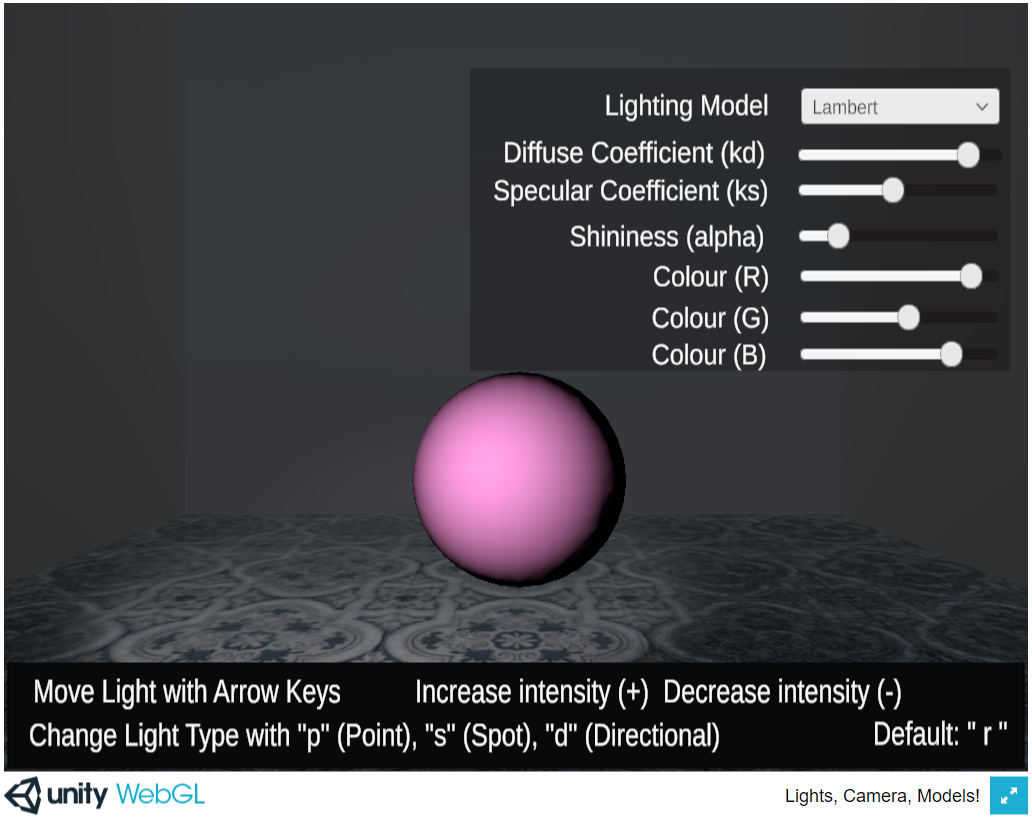
\includegraphics[scale=0.25]{./images/sphere-lit-lambert}
	\caption{Default Scene for \famname}
\end{figure}


\paragraph{Lighting Model Changes}

\begin{enumerate}

	\item{lightModel-ModLambert\\}

	Control: Manual
	
	Input: Select Mod-Lambert lighting model from dropdown list.
	
	Output: Scene render with Mod-Lambert lit sphere.
	
	\begin{figure}[h]
		\centering
		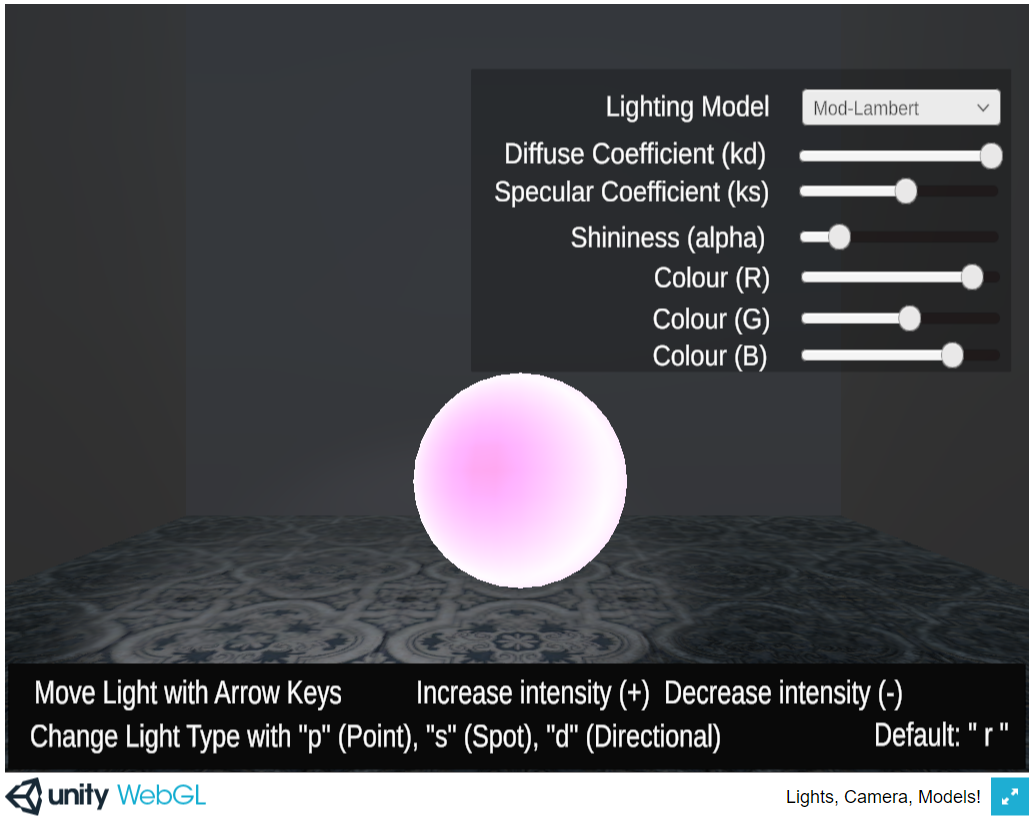
\includegraphics[scale=0.25]{./images/sphere-lit-modlambert}
		\caption{Default Scene with Lighting Model changed to Mod-Lambert}
		\label{fig:modLambert}
	\end{figure}
	
	Test Case Derivation: After a scene is loaded, the user can only interact 
	with the system through its GUI. Lighting model changes are determined by 
	dropdown list selection. The scene default is to have a sphere lit with the 
	Lambert (Diffuse) lighting model; changing to the Mod-Lambert will make a 
	significant difference and should be easily noticeable as most of the 
	shadows disappear.
	
	How test will be performed: System will recalculate luminous intensity of 
	points on objects in the scene using the new model. New luminous intensity 
	information will be sent through the rendering pipeline to output        
	visuals. Tester will visually compare whether output matches the image 
	provided here.
	
	\item{lightModel-Phong\\}
	
	Control: Manual
	
	Input: Select Phong lighting model from dropdown list. 
	
	Output: Scene render with Phong lit sphere.
	
	\begin{figure}[h]
		\centering
		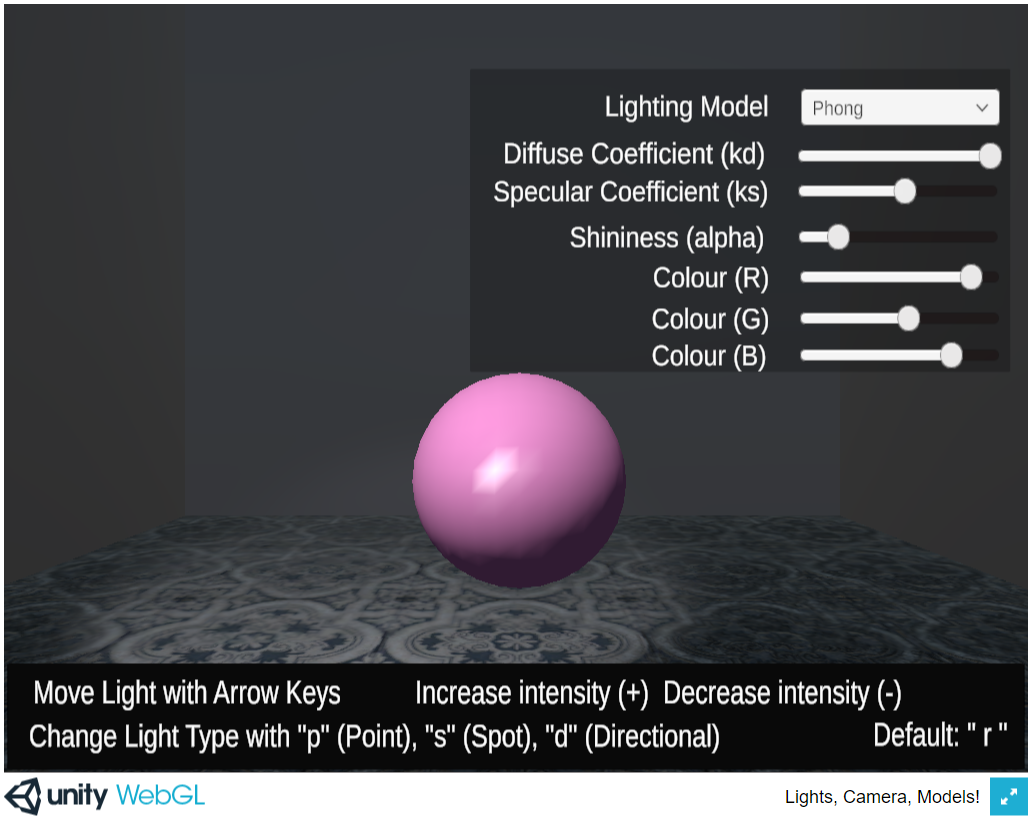
\includegraphics[scale=0.25]{./images/sphere-lit-phong}
		\caption{Default Scene with Lighting Model changed to Phong}
		\label{fig:Phong}
	\end{figure}
	
	Test Case Derivation: After a scene is loaded, the user can only interact 
	with the system through its GUI. Lighting model changes are determined by 
	dropdown list selection. The scene default is to have a sphere lit with the 
	Lambert (Diffuse) lighting model; changing to the Phong will make a 
	significant difference and should be easily noticeable.
	
	How test will be performed: System will recalculate luminous intensity of 
	points on objects in the scene using the new model. New luminous intensity 
	information will be sent through the rendering pipeline to output        
	visuals. Tester will visually compare whether output matches the image 
	provided here.
	
	\item{lightModel-BlinnPhong\\}
	
	Control: Manual
	
	Input: Select Blinn-Phong lighting model from dropdown list. \wss{There
          isn't enough information here for someone else to do this test.  The
          input is ambiguous.  The same comment applies for other tests in this
          section.}
	
	Output: Scene render with Blinn-Phong lit sphere.
	
	\begin{figure}[h]
		\centering
		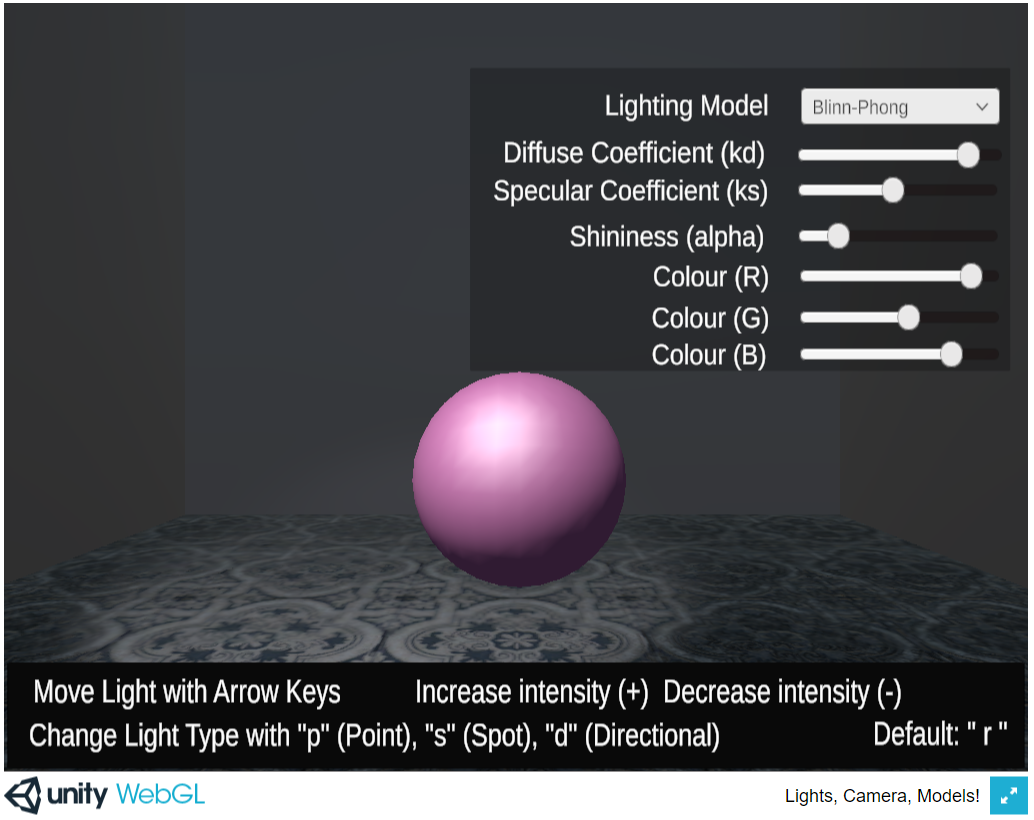
\includegraphics[scale=0.25]{./images/sphere-lit-blinnphong}
		\caption{Default Scene with Lighting Model changed to Blinn-Phong}
		\label{fig:blinnPhong}
	\end{figure}
	
	Test Case Derivation: After a scene is loaded, the user can only interact 
	with the system through its GUI. Lighting model changes are determined by 
	dropdown list selection. The scene default is to have a sphere lit with the 
	Lambert (Diffuse) lighting model; changing to the Blinn-Phong will make a 
	significant difference and should be easily noticeable.
	
	How test will be performed: System will recalculate luminous intensity of 
	points on objects in the scene using the new model. New luminous intensity 
	information will be sent through the rendering pipeline to output        
	visuals. Tester will visually compare whether output matches the image 
	provided here. \wss{How do you tell if this test has passed?  How do you 
	tell
          this automatically?}
	
\end{enumerate}

%\paragraph{Shading Model Changes}
%
%\begin{enumerate}
%	
%	\item{shadingModel-valid\\}
%	
%	Control: Automatic
%	
%	Input: Select different shading model from dropdown list.
%	
%	Output: \textit{RENDERS\_DIR/render-valid-AllInputs} with visuals based on 
%	new shading models.
%	
%	Test Case Derivation: After a scene is loaded, the user can only interact 
%	with the system through its GUI. Shading model changes are determined by 
%	dropdown list selection.
%	
%	How test will be performed: System will recalculate surface normals of 
%	points on objects in the scene using the new model. New surface normal
%	information will be sent through the rendering pipeline to output visuals.
%	
%\end{enumerate}

\paragraph{Object Changes}

\begin{enumerate}
%%Object Material Properties
%Valid changes	
	\item{objMaterialPropChange-valid-ks\\}
	
	Control: Manual
	
	Initial State: Default Scene with lighting model set to Blinn-Phong (see 
	\ref{fig:blinnPhong})
	
	Input: $k_{s} = 1$
	
	Output: Scene render with Blinn-Phong lit and brighter and larger specular 
	reflection.
	
	\begin{figure}[h]
		\centering
		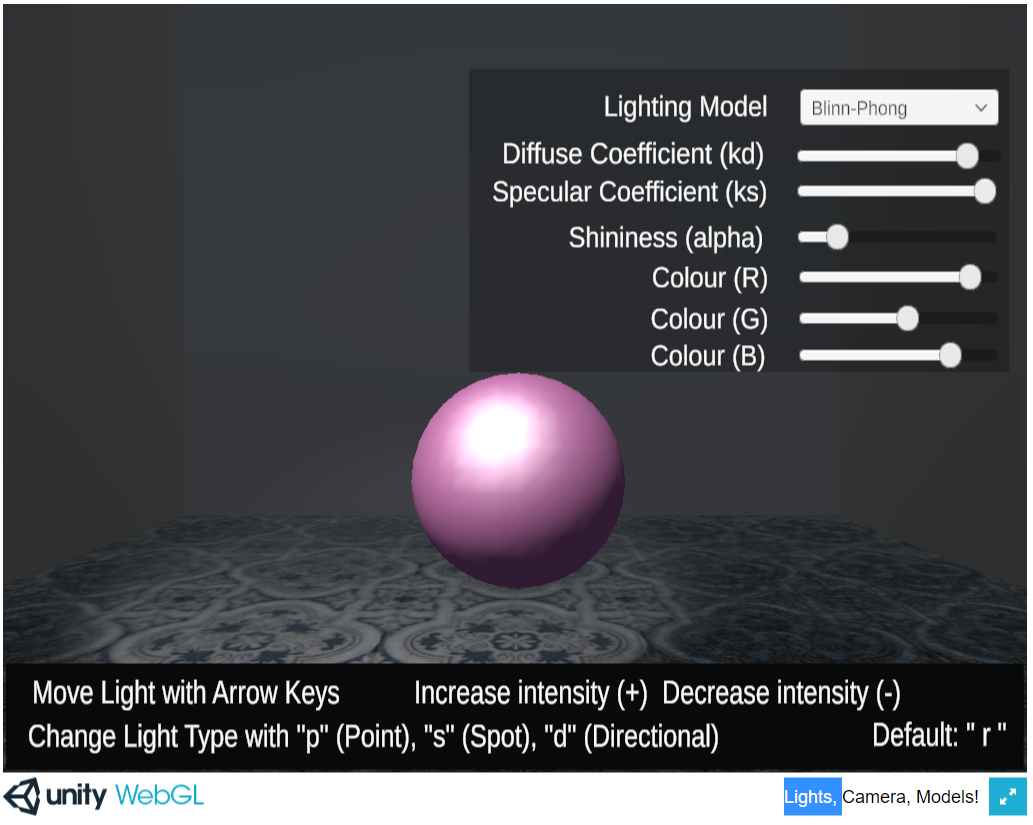
\includegraphics[scale=0.25]{./images/sphere-lit-blinnphong-ks1}
		\caption{Default Scene with Lighting Model changed to Blinn-Phong and 
		$k_{s}$ set to 1}
		\label{fig:blinnPhong-ks1}
	\end{figure}
	
	Test Case Derivation: $I_{s} = k_{s}\cdot i(p,p_{0}) \cdot \max(0, 
	({L_{r}}\bullet V))^\alpha$. Final colouring of any point in a scene is 
	$(I_{a}+I_{d}+I_{s})\cdot LIGHT\_COLOUR$, therefore changes to the $k_{s}$ 
	impact the specular component of the final scene.
	
	How test will be performed: Default scene is loaded. Testing framework 
	automatically assigns $k_{s}$ the new value. Tester manually checks the 
	output images to compare the change in specular reflection. \wss{How do you
          automatically tell that this test case passes?  Are you just checking
          a single value, or how the value is used in the scene?  A similar
          comment applies to other test cases in this section.}
	
	\item{objMaterialPropChange-valid-kd\\}
	
	Control: Manual
	
	Input: $k_{d} = 0.5$
	
	Output: Scene render with Blinn-Phong lit, with colour of sphere being dull.
	\begin{figure}[h]
		\centering
		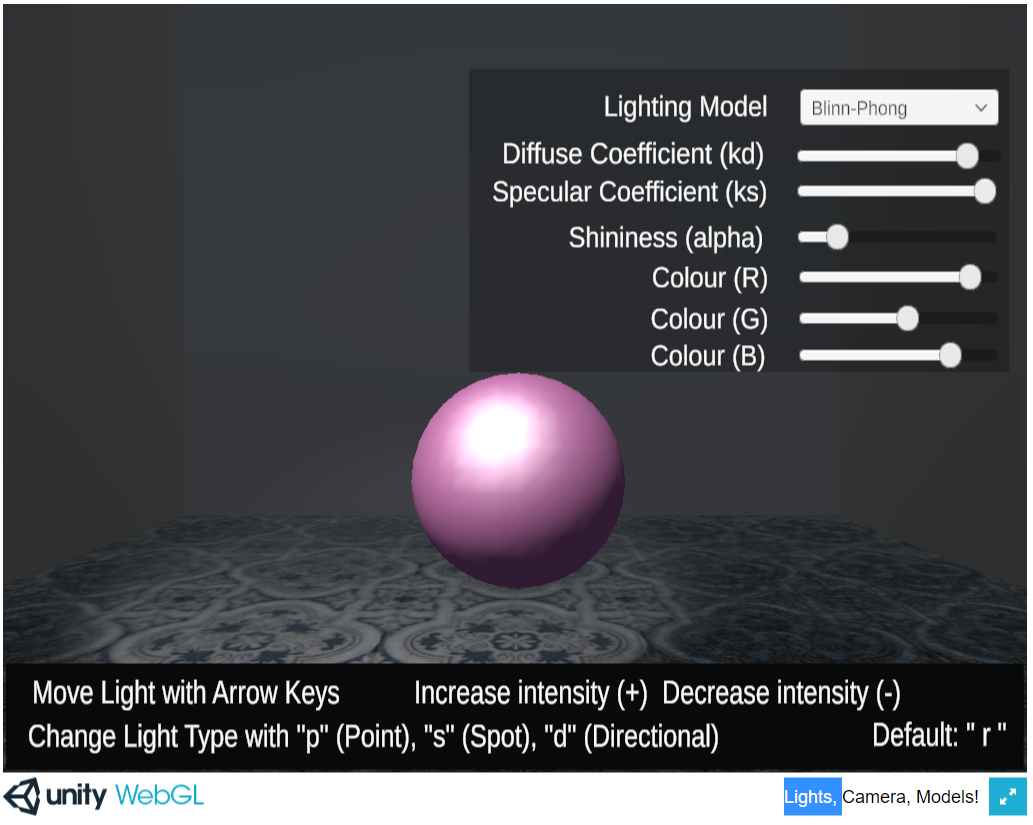
\includegraphics[scale=0.25]{./images/sphere-lit-blinnphong-ks1}
		\caption{Default Scene with Lighting Model changed to Blinn-Phong and 
			$k_{s}$ set to 1}
		\label{fig:blinnPhong-kd0.5}
	\end{figure}	
	
	
	Test Case Derivation: $I_{d} = k_{d}\cdot i(p,p_{0}) \cdot 
	\max(0,(L_{i}\bullet N))$. Final colouring of any point in a scene is 
	$(I_{a}+I_{d}+I_{s})\cdot LIGHT\_COLOUR$, therefore changes to the $k_{d}$ 
	impact the diffuse component of the final scene.
	
	How test will be performed: Valid scene is loaded. Testing framework 
	automatically assigns $k_{d}$ the new value. 	

\sms{Tests for changing $k_{a}$ have been removed as this coefficient does not 
affect the calculations for the models chosen and so has not been implemented.}
%	\item{objMaterialPropChange-valid-ka\\}
%	
%	Control: Automatic
%	
%	Input: $k_{a} = 0.5$
%	
%	Output: \textit{RENDERS\_DIR/render-valid-AllInputs} with visuals changed 
%	so that specular reflection uses new value.
%	
%	Test Case Derivation: $I_{a} = k_{a}\cdot i(p,p_{0})$. Final colouring of 
%	any point in a scene is $(I_{a}+I_{d}+I_{s})\cdot LIGHT\_COLOUR$, therefore 
%	changes to the $k_{a}$ impact the ambient component of the final scene.
%	
%	How test will be performed: Valid scene is loaded. Testing framework 
%	automatically assigns $k_{a}$ the new value. 
%
%	\item{objMaterialPropChange-valid-$\alpha$\\}
%	
%	Control: Automatic
%	
%	Input: $\alpha = 2$
%	
%	Output: \textit{RENDERS\_DIR/render-valid-AllInputs} with visuals changed 
%	so that specular reflection uses new value.
%	
%	Test Case Derivation: $I_{s} = k_{s}\cdot i(p,p_{0}) \cdot \max(0, 
%	({L_{r}}\bullet V))^\alpha$. Final colouring of any point in a scene is 
%	$(I_{a}+I_{d}+I_{s})\cdot LIGHT\_COLOUR$, therefore changes to the $\alpha$ 
%	impact the specular component of the final scene.
%	
%	How test will be performed: Valid scene is loaded. Testing framework 
%	automatically assigns $\alpha$ the new value. 

	\item{objMaterialPropChange-valid-$\alpha$\\}

	Control: Manual
	
	Input: $\alpha = 100$
	
	Output: Scene render of Blinn-Phong lit sphere and smaller sharper specular 
	reflection.
	\begin{figure}[h]
	\centering
		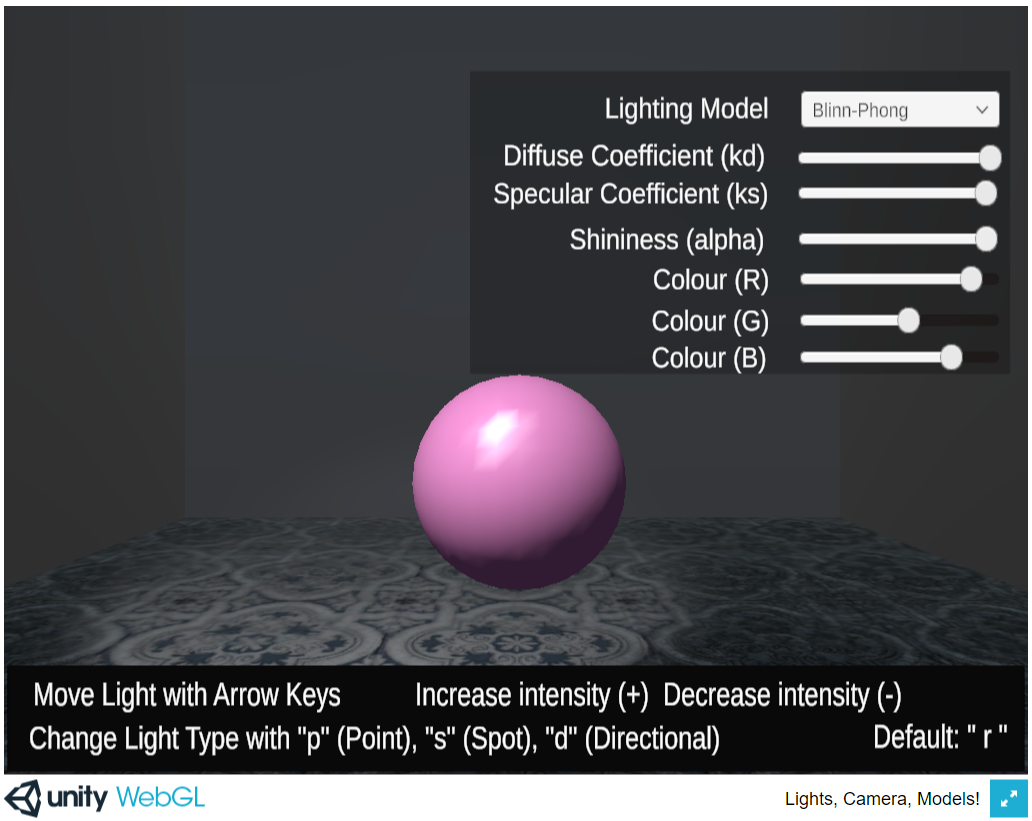
\includegraphics[scale=0.25]{./images/sphere-lit-blinnphong-a100}
		\caption{Default Scene with Lighting Model changed to Blinn-Phong and 
			$\alpha$ set to 100}
		\label{fig:blinnPhong-a100}
	\end{figure}		
	
	
	Test Case Derivation: 
	
	How test will be performed: Valid scene is loaded. Testing framework 
	attempts to assign $\alpha$ the new value. 

As the changes to the material property values are determined by sliders, it is 
impossible for a user to input an invalid value for these properties. As such 
there are no ``invalid input'' tests.
%%Invalid
%	\item{objMaterialPropChange-invalid-ks\\}
%	
%	Control: Automatic
%	
%	Input: $k_{s} = 2$
%	
%	Output: Error Message ``New value of $k_{s}$ is outside of bounds. Please 
%	enter a different value.''. Log message ``Error: tried to assign $k_{s} = 
%	2$''. 
%	
%	Test Case Derivation: $0 \le k_{s} \le 1$; therefore the new assignment is 
%	invalid by the constraints.
%	
%	How test will be performed: Valid scene is loaded. Testing framework 
%	attempts to assign $k_{s}$ the new value. Error message is loaded instead. 
%	Error is written to log file.
%	
%	\item{objMaterialPropChange-invalid-kd\\}
%	
%	Control: Automatic
%	
%	Input: $k_{d} = 2$
%	
%	Output: Error Message ``New value of $k_{d}$ is outside of bounds. Please 
%	enter a different value.''. Log message ``Error: tried to assign $k_{d} = 
%	2$''. 
%	
%	Test Case Derivation: $0 \le k_{d} \le 1$; therefore the new assignment is 
%	invalid by the constraints.
%	
%	How test will be performed: Valid scene is loaded. Testing framework 
%	attempts to assign $k_{d}$ the new value. Error message is loaded instead. 
%	Error is written to log file.
%	
%	\item{objMaterialPropChange-invalid-ka\\}
%	
%	Control: Automatic
%	
%	Input: $k_{a} = 2$
%	
%	Output: Error Message ``New value of $k_{a}$ is outside of bounds. Please 
%	enter a different value.''. Log message ``Error: tried to assign $k_{a} = 
%	2$''. 
%	
%	Test Case Derivation: $0 \le k_{a} \le 1$; therefore the new assignment is 
%	invalid by the constraints.
%	
%	How test will be performed: Valid scene is loaded. Testing framework 
%	attempts to assign $k_{a}$ the new value. Error message is loaded instead. 
%	Error is written to log file.
%
%	\item{objMaterialPropChange-invalid-$\alpha$\\}
%	
%	Control: Automatic
%	
%	Input: $\alpha = -2$
%	
%	Output: Error Message ``New value of $\alpha$ is outside of bounds. Please 
%	enter a different value.''. Log message ``Error: tried to assign $\alpha = 
%	-2$''. 
%	
%	Test Case Derivation: $\alpha : \mathbb{Z_{+}}$; therefore the new 
%	assignment 
%	is invalid by the constraints.
%	
%	How test will be performed: Valid scene is loaded. Testing framework 
%	attempts to assign $\alpha$ the new value. Error message is loaded instead. 
%	Error is written to log file.

\sms{Boundary condition test cases have been removed as they are used in the 
valid input test cases. As such the valid input test cases both function to 
check the correctness of the final render, but also how the system reacts to 
the boundary values of its parameters.}
%Boundary	
%	\item{objMaterialPropChange-bound-ks\\}
%	
%	Control: Automatic
%	
%	Input: $k_{s} = 1$
%	
%	Output: \textit{RENDERS\_DIR/render-valid-AllInputs} with visuals changed 
%	so that specular reflection uses new value.
%	
%	Test Case Derivation: $I_{s} = k_{s}\cdot i(p,p_{0}) \cdot \max(0, 
%	({L_{r}}\bullet V))^\alpha$. Final colouring of any point in a scene is 
%	$(I_{a}+I_{d}+I_{s})\cdot LIGHT\_COLOUR$, therefore changes to the $k_{s}$ 
%	impact the specular component of the final scene.
%	
%	How test will be performed: Valid scene is loaded. Testing framework 
%	automatically assigns $k_{s}$ the new value. 
%	
%	\item{objMaterialPropChange-bound-kd\\}
%	
%	Control: Automatic
%	
%	Input: $k_{d} = 1$
%	
%	Output: \textit{RENDERS\_DIR/render-valid-AllInputs} with visuals changed 
%	so that specular reflection uses new value.
%	
%	Test Case Derivation: $I_{d} = k_{d}\cdot i(p,p_{0}) \cdot 
%	\max(0,(L_{i}\bullet N))$. Final colouring of any point in a scene is 
%	$(I_{a}+I_{d}+I_{s})\cdot LIGHT\_COLOUR$, therefore changes to the $k_{d}$ 
%	impact the diffuse component of the final scene.
%	
%	How test will be performed: Valid scene is loaded. Testing framework 
%	automatically assigns $k_{d}$ the new value. 	
%	
%	\item{objMaterialPropChange-bound-ka\\}
%	
%	Control: Automatic
%	
%	Input: $k_{a} = 1$
%	
%	Output: \textit{RENDERS\_DIR/render-valid-AllInputs} with visuals changed 
%	so that specular reflection uses new value.
%	
%	Test Case Derivation: $I_{a} = k_{a}\cdot i(p,p_{0})$. Final colouring of 
%	any point in a scene is $(I_{a}+I_{d}+I_{s})\cdot LIGHT\_COLOUR$, therefore 
%	changes to the $k_{a}$ impact the ambient component of the final scene.
%	
%	How test will be performed: Valid scene is loaded. Testing framework 
%	automatically assigns $k_{a}$ the new value. 
%	
%	\item{objMaterialPropChange-bound-$\alpha$\\}
%	
%	Control: Automatic
%	
%	Input: $\alpha = 0$
%	
%	Output: \textit{RENDERS\_DIR/render-valid-AllInputs} with visuals changed 
%	so that specular reflection uses new value.
%	
%	Test Case Derivation: $I_{s} = k_{s}\cdot i(p,p_{0}) \cdot \max(0, 
%	({L_{r}}\bullet V))^\alpha$. Final colouring of any point in a scene is 
%	$(I_{a}+I_{d}+I_{s})\cdot LIGHT\_COLOUR$, therefore changes to the $\alpha$ 
%	impact the specular component of the final scene.
%	
%	How test will be performed: Valid scene is loaded. Testing framework 
%	automatically assigns $\alpha$ the new value.

\sms{Tests relating to object size and position have been removed as the 
functionality to change these properties of the object no longer exist.}
%%%Object Position	
%%Valid
%	\item{objPosition-valid\\}
%	
%	Control: Automatic
%	
%	Input: New Point (2,0,0) for centre of object
%	
%	Output: \textit{RENDERS\_DIR/render-valid-AllInputs} with visuals changed 
%	to reflect object movement to coordinate (2,0,0) (including update of 
%	lighting as distance from light source is changed).
%	
%	Test Case Derivation: Lighting is dependent of position of object relative 
%	to the light source; therefore movement in position changes the lighting of 
%	an object causing all the intensities to be recalculated and the object to 
%	be recoloured.
%
%	How test will be performed: Valid scene is loaded. Testing framework 
%	automatically assigns new position to (2,0,0). System recalculates 
%	intensities and recolours moved object.
%	
%%Invalid	
%	\item{objPosition-invalid-outBounds\\}
%	
%	Control: Automatic
%	
%	Input: New Point (11,0,0) for centre of object
%	
%	Output: Error Message ``The centre of this object is outside of the room. 
%	It cannot be rendered. Please enter a different location for this 
%	object.''. Log message ``Error: Tried to move centre of object to (11,0,0).
%	
%	Test Case Derivation: Scene size is defined to be (SCENE\_HEIGHT, 
%	SCENE\_WIDTH, SCENE\_DEPTH); if any component of the object's position is 
%	greater than any component of the scene size then the object is out of 
%	bounds. Out of bounds objects cannot be lit or rendered.
%	
%	How test will be performed: Valid scene is loaded. Testing framework 
%	automatically assigns new position to (11,0,0). System throws an error.
%	
%	\item{objPosition-invalid-onLight\\}
%	
%	Control: Automatic
%	
%	Input: New Point (5,5,5) for centre of object
%	
%	Output: Error Message ``The centre of this object intersects the light 
%	source.	It cannot be rendered. Please enter a different location for this 
%	object.''. Log message ``Error: Tried to move centre of object to light 
%	source position, (5,5,5)''.
%	
%	Test Case Derivation: As per the requirement (\ref) objects cannot be on 
%	top of the light source. This would create a design issue of whether the 
%	opaque object would be blocking the light. To circumvent this, we impose 
%	that they cannot have their centres at the same position.
%	
%	How test will be performed: Valid scene is loaded. Testing framework 
%	automatically assigns new position to (5,5,5). System throws an error.
%
%	\item{objPosition-invalid-onObserver\\}
%	
%	Control: Automatic
%	
%	Input: New Point (0,0,0) for centre of object
%	
%	Output: Error Message ``The centre of this object intersects the observer.	
%	It cannot be rendered. Please enter a different location for this 
%	object.''. Log message ``Error: Tried to move centre of object to observer 
%	position, (0,0,0)''.
%	
%	Test Case Derivation: As per the requirement (\ref) objects cannot be on 
%	top of the observer. This would create a design issue of whether the 
%	opaque object would be blocking the view, and how it would be lit. To 
%	circumvent this, we impose that they cannot have their centres at the same 
%	position.
%	
%	How test will be performed: Valid scene is loaded. Testing framework 
%	automatically assigns new position to (0,0,0). System throws an error.
%	
%%Boundary		
%	\item{objPosition-valid-edgeOfRoom\\}
%	
%	Control: Automatic
%	
%	Input: New Point (0,10,0) for centre of object
%	
%	Output: Error Message ``Parts of this object are outside of the scene size. 
%	Please move this object and re-render the scene.''. Log Message ``Error: 
%	Object partially outside of room.''
%	
%	Test Case Derivation: Constraints on object position said $0 \ll 
%	x \le SIZE\_HEIGHT$, which means that the centre is on the wall of the 
%	scene. This means part of the object would be rendered outside the scene.
%	
%	How test will be performed: Valid scene is loaded. Testing framework 
%	automatically assigns new position to (0,10,0). System throws an error.
%
%	\item{objPosition-valid-betweenLightAndViewer\\}
%	
%	Control: Automatic
%	
%	Input: New Point (2,2,2) for centre of object
%	
%	Output: \textit{RENDERS\_DIR/render-valid-AllInputs} with visuals changed 
%	to reflect object movement to coordinate (2,2,2) (including update of 
%	lighting as distance from light source is changed).
%	
%	Test Case Derivation: Lighting is dependent of position of object relative 
%	to the light source; therefore movement in position changes the lighting of 
%	an object causing all the intensities to be recalculated and the object to 
%	be recoloured. When an object is between the light and the viewer its faces 
%	should be dark as they're not being lit.
%	
%	How test will be performed: Valid scene is loaded. Testing framework 
%	automatically assigns new position to (2,2,2). System recalculates 
%	intensities and recolours moved object.	
%	
%	\item{objPosition-valid-besideLight\\}
%	
%	Control: Automatic
%	
%	Input: New Point (5,3,0) for centre of object
%	
%	Output: \textit{RENDERS\_DIR/render-valid-AllInputs} with visuals changed 
%	to reflect object movement to coordinate (5,3,0) (including update of 
%	lighting as distance from light source is changed).
%	
%	Test Case Derivation: Lighting is dependent of position of object relative 
%	to the light source; therefore movement in position changes the lighting of 
%	an object causing all the intensities to be recalculated and the object to 
%	be recoloured. When an object is beside a light source it is highly 
%	illuminated making it very bright.
%	
%	How test will be performed: Valid scene is loaded. Testing framework 
%	automatically assigns new position to (5,3,0). System recalculates 
%	intensities and recolours moved object.			

%%Object Colour
	\item{objColour-valid-base\\}
	
	Control: Automatic
	
	Input: New (r,g,b) value for BASE\_COLOUR picked from GUI picker = 
	(0,0,0).
	
	Output: Scene render of Blinn-Phong with a black object material. All 
	diffuse terms need to be recalculated.
	
	\begin{figure}[h]
		\centering
		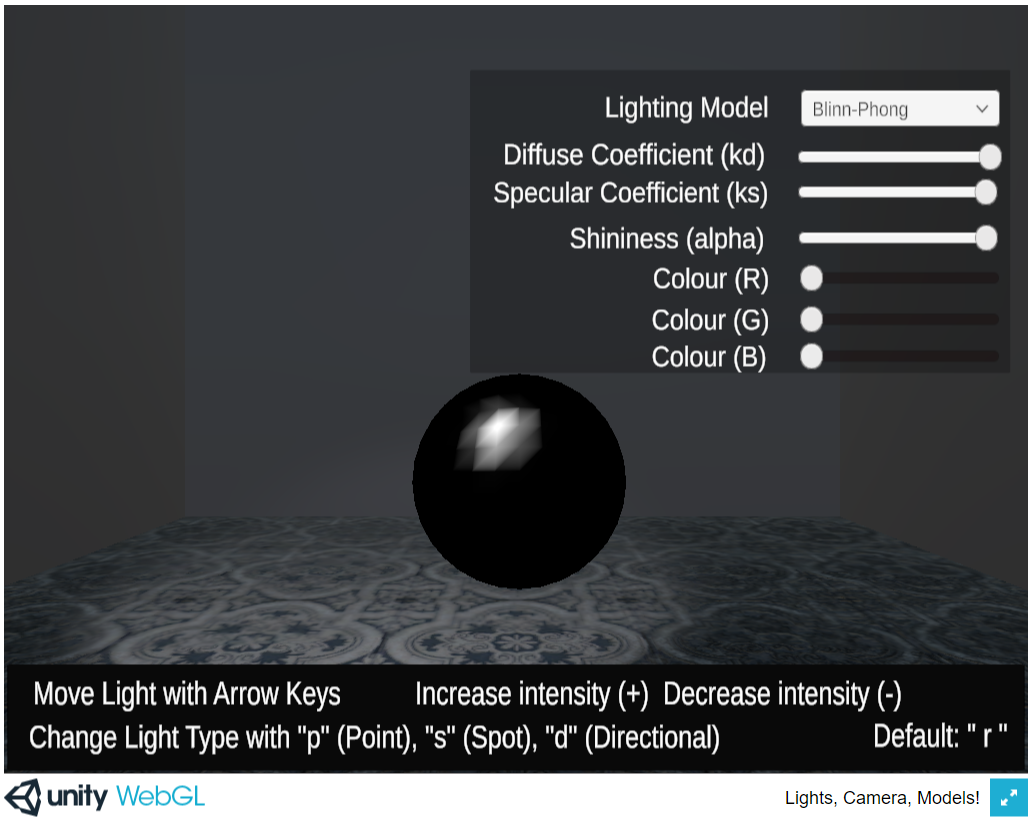
\includegraphics[scale=0.25]{./images/sphere-lit-blinnphong-colour}
		\caption{Default Scene with Lighting Model changed to Blinn-Phong and 
			BASE\_COLOUR set to (0,0,0)}
		\label{fig:blinnPhong-black}
	\end{figure}	
	
	Test Case Derivation: The BASE\_COLOUR at a point is part 
	of the all lighting model calculations. Change the BASE\_COLOUR requires 
	recalculating all of the intensity values with this new (r,g,b) information.
	
	How test will be performed: Valid scene is loaded. Testing framework 
	automatically assigns new r,g,b to (0,0,0). System recalculates 
	intensities and recolours object.			

\sms{Removed test for specular colour change because we have it set to 
exclusively be white.}
%	\item{objColour-valid-specular\\}
%	
%	Control: Automatic
%	
%	Input: New (r,g,b) value for SPECULAR\_COLOUR picked from GUI picker = 
%	(10,255,50).
%	
%	Output: \textit{RENDERS\_DIR/render-valid-AllInputs} with visuals changed 
%	to reflect the new base colour for the object. All diffuse terms need to be 
%	recalculated.
%	
%	Test Case Derivation: The intensity of the SPECULAR\_COLOUR at a point is 
%	part of the specular component calculation. Change the SPECULAR\_COLOUR 
%	requires recalculating all of the intensity values with this new (r,g,b) 
%	information.
%	
%	How test will be performed: Valid scene is loaded. Testing framework 
%	automatically assigns new r,g,b to (10,255,50). System recalculates 
%	intensities and recolours object.	
%	

\sms{Shape changing feature has been removed from current implementation. This 
test case has been commented out as this feature is top priority to return 
after the course is complete.}
%	\item{objShape-valid\\}
%	
%	Control: Automatic
%	
%	Input: New shape selection from dropdown list: torus.
%	
%	Output: \textit{RENDERS\_DIR/render-valid-AllInputs} with visuals changed 
%	to replace the sphere with a torus. All normals have changed, so all 
%	intensities need to be recalculated.
%	
%	Test Case Derivation: Different shapes have different normals, and so 
%	different ways of reflecting. The models need  to be sure to work with not 
%	just a sphere, but other objects as well.
%	
%	How test will be performed: Valid scene is loaded. Testing framework 
%	automatically assigns new object shape. System recalculates 
%	intensities and recolours new object.
			
\end{enumerate}

\paragraph{Light Changes}

\begin{enumerate}
%%Light Positions
%Valid
	\item{lightPos-valid\\}
	
	Control: Manual
	
	Input: \\
	\textit{Variation 1}: Light Type = Spotlight, Press left arrow 5 times\\
	\textit{Variation 2}: Light Type = Point Light, Press left arrow key 5 
	times\\
	\textit{Variation 3}: Light Type = Directional, Press right arrow key 5 
	times\\
	\textit{Variation 4}: Light Type = Spotlight, Press right arrow key 10
	times\\
	\textit{Variation 5}: Light Type = Point Light, Press right arrow key 10
	times\\
	
	Output: Scene render based on new position of light source.

	\begin{figure}[h]
	\centering
	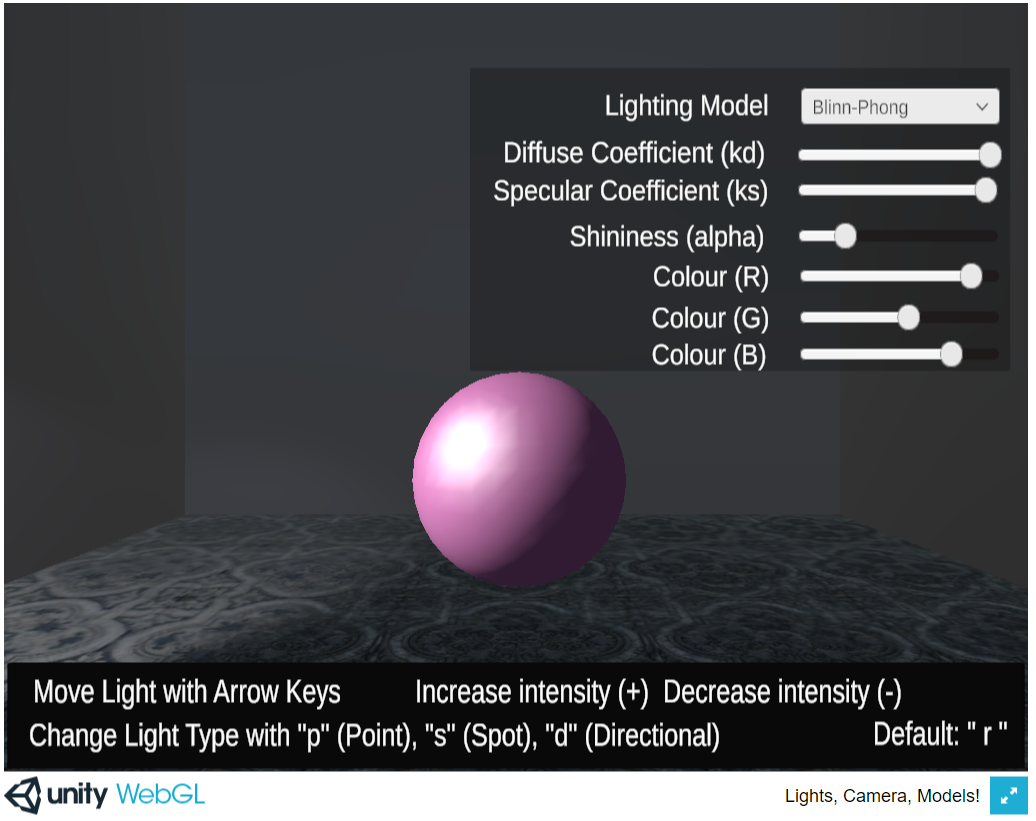
\includegraphics[scale=0.25]{./images/sphere-lit-spotlight-moveValid}
	\caption{Output Variation 1}
	\label{fig:spotlight-move}
	\end{figure}	
	
	\begin{figure}[h]
		\centering
		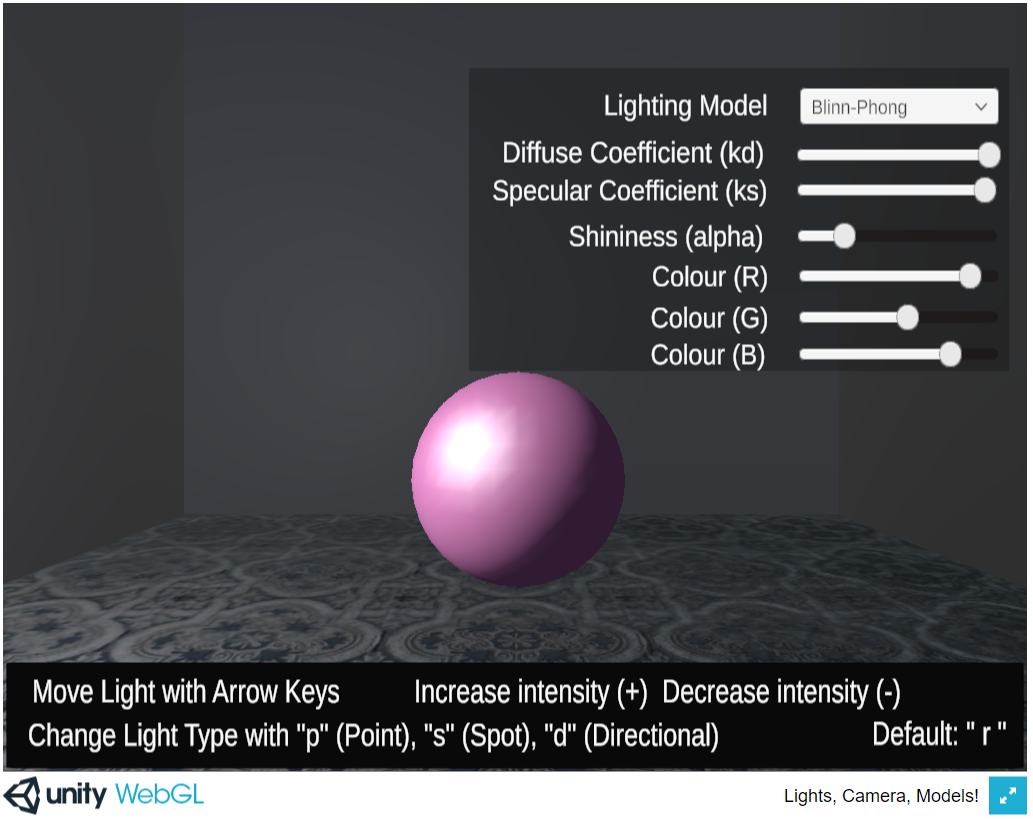
\includegraphics[scale=0.25]{./images/sphere-lit-point-moveValid}
		\caption{Output Variation 2}
		\label{fig:point-move}
	\end{figure}	
	
	\begin{figure}[h]
		\centering
		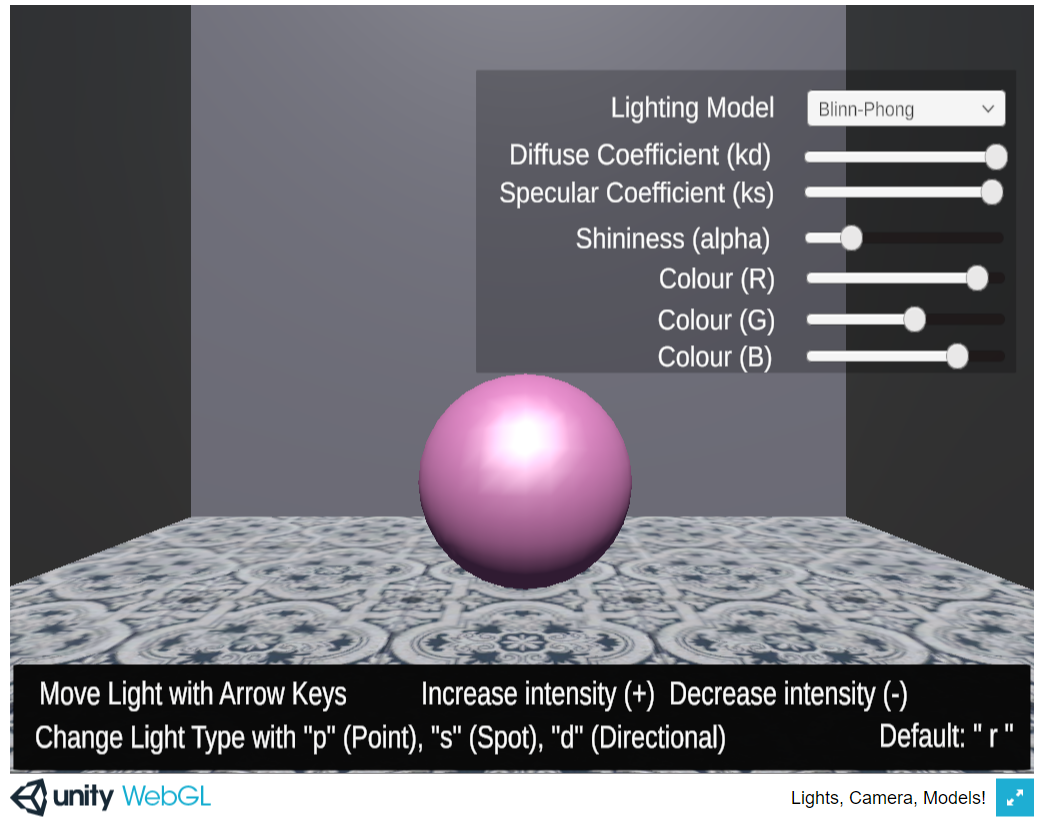
\includegraphics[scale=0.25]{./images/sphere-lit-direction}
		\caption{Output Variation 3}
		\label{fig:directional-move}
	\end{figure}

	\begin{figure}[h]
	\centering
	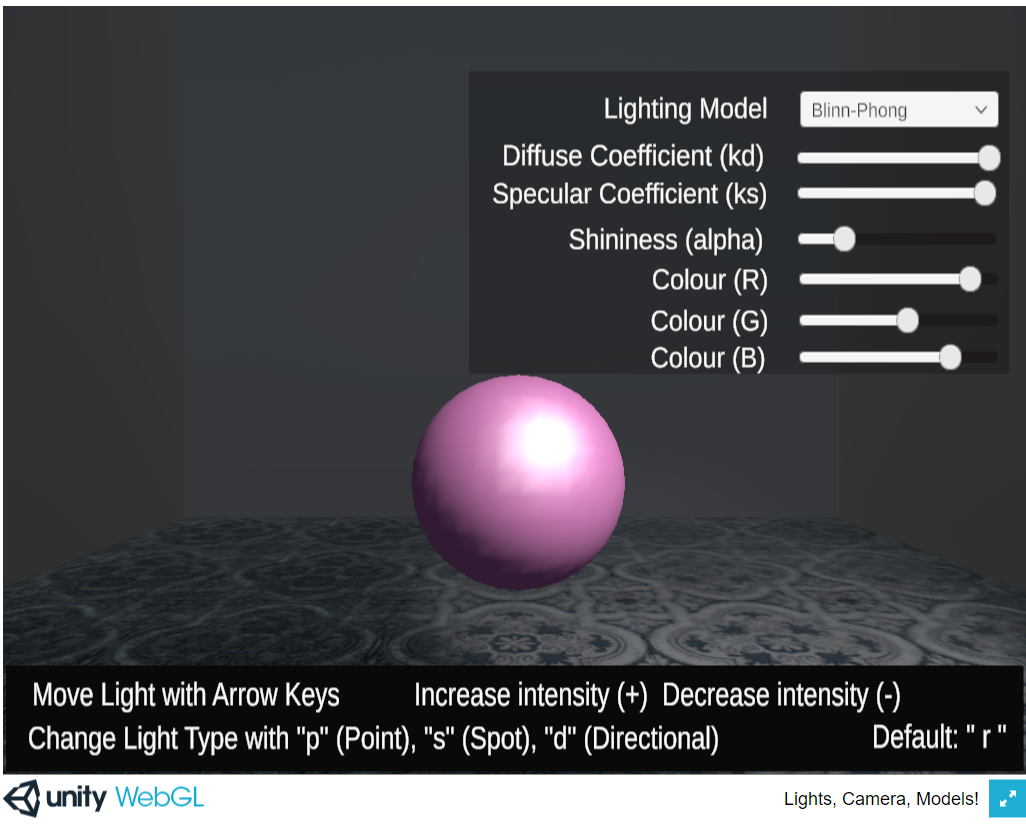
\includegraphics[scale=0.25]{./images/sphere-lit-spotlight-moveValidR}
	\caption{Output Variation 4}
	\label{fig:spotlight-move-right}
	\end{figure}	
	
	\begin{figure}[h]
		\centering
		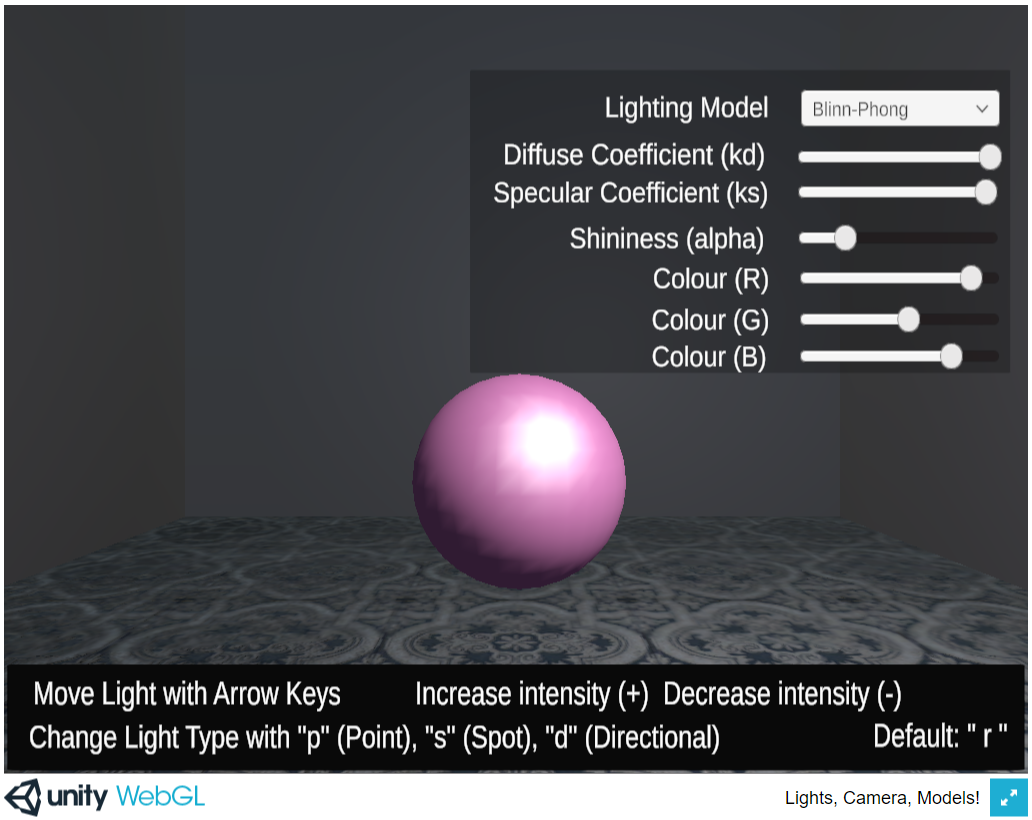
\includegraphics[scale=0.25]{./images/sphere-lit-point-moveValidR}
		\caption{Output Variation 5}
		\label{fig:point-move-right}
	\end{figure}	

	
	Test Case Derivation: Lighting is dependent of position of object relative 
	to the light source; therefore movement in light source position changes 
	the lighting of objects causing all the intensities to be recalculated and 
	the object to be recoloured.
	
	How test will be performed: Valid scene is loaded. Testing framework 
	automatically assigns new position to (2,0,0). System recalculates 
	intensities and recolours moved object.
	
%%Invalid	
%	\item{lightPos-invalid-outBounds\\}
%	
%	Control: Automatic
%	
%	Input: New Point (11,0,0) for centre of light
%	
%	Output: Error Message ``This light source is outside of the room. It cannot 
%	be rendered. Please enter a different location for this object.''. Log 
%	message ``Error: Tried to move light source to (11,0,0).
%	
%	Test Case Derivation: Scene size is defined to be (SCENE\_HEIGHT, 
%	SCENE\_WIDTH, SCENE\_DEPTH); if any component of the light source's 
%	position is greater than any component of the scene size then the light 
%	source is out of bounds. Out of bounds light sources cannot light the scene.
%	
%	How test will be performed: Valid scene is loaded. Testing framework 
%	automatically assigns new position to (11,0,0). System throws an error.
%	
\sms{Object and Light are locked at different values of the z-plane, with no 
way for the light to traverse between them. Therefore the light can never end 
up on the object and so this test case has been omitted.}
%	\item{lightPos-invalid-onObj\\}
%	
%	Same as \textit{objPosition-invalid-onLight}.
%	
%	\item{lightPos-invalid-onObserver\\}
%	
%	Control: Automatic
%	
%	Input: New Point (0,0,0) for centre of light source.
%	
%	Output: Error Message ``The centre of this light source intersects the 
%	observer. It cannot be rendered. Please enter a different location for this 
%	object.''. Log message ``Error: Tried to move light source to observer 
%	position, (0,0,0)''.
%	
%	Test Case Derivation: As per the requirement (\ref) light sources cannot be 
%	on top of the observer. We impose that they cannot have their centres at 
%	the same position.
%	
%	How test will be performed: Valid scene is loaded. Testing framework 
%	automatically assigns new position to (0,0,0). System throws an error.

%Boundary	
\sms{The boundary conditions check and enforce that the light cannot move 
outside of the scene room in the code. As such, checking the boundary cases 
here should ensure that no invalid values are allowed.}
	\item{lightPos-boundaries\\}
	
	Control: Manual
	
	Input:  \\
	\textit{Variation 1}: Light Type = Spotlight, Press right arrow key 31 
	times\\
	\textit{Variation 2}: Light Type = Point Light, Press right arrow key 31 
	times\\
	\textit{Variation 3}: Light Type = Directional, Press right arrow key 31 
	times\\
	\textit{Variation 4}: Light Type = Spotlight, Press left arrow key 20 
	times\\
	\textit{Variation 5}: Light Type = Point Light, Press left arrow key 20 
		times\\
		
	Output: Scene render and lit with Blinn-Phong lighting model, and 
	reflections changing depending on the position of the light.
	
	\begin{figure}[h]
		\centering
		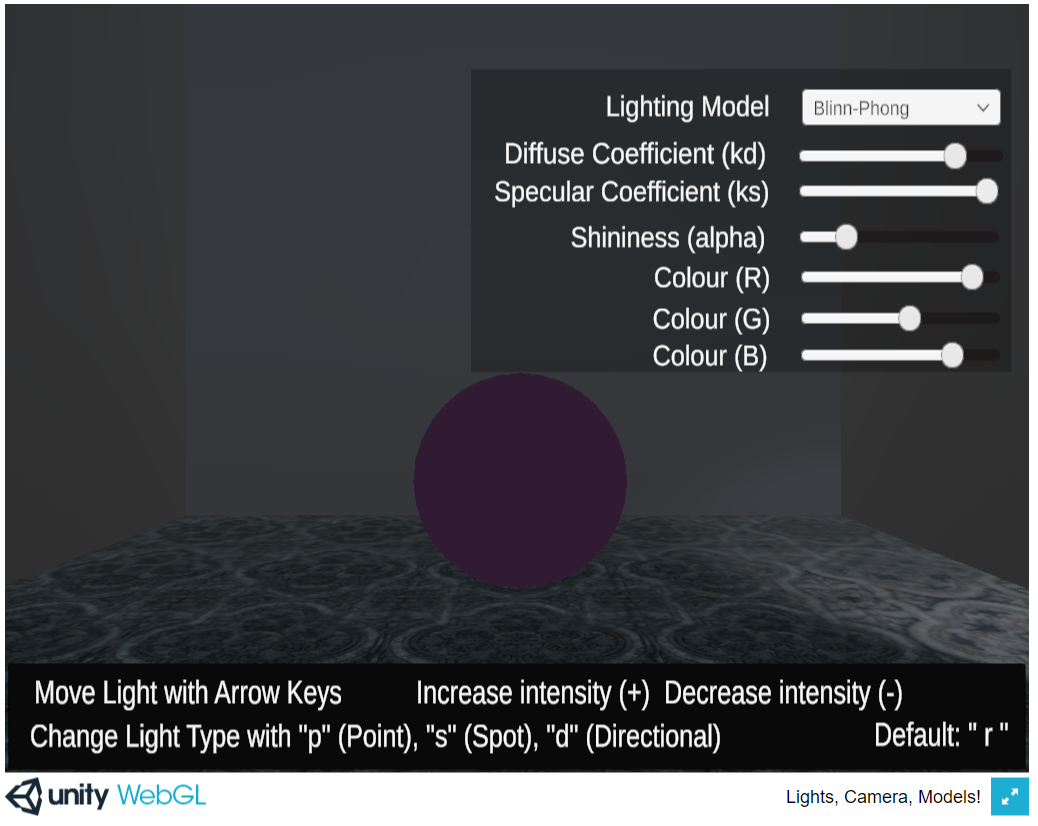
\includegraphics[scale=0.25]{./images/sphere-lit-spotlight-moveBoundsR}
		\caption{Output Variation 1}
		\label{fig:spotlight-bounds-right}
	\end{figure}	

	\begin{figure}[h]
		\centering
		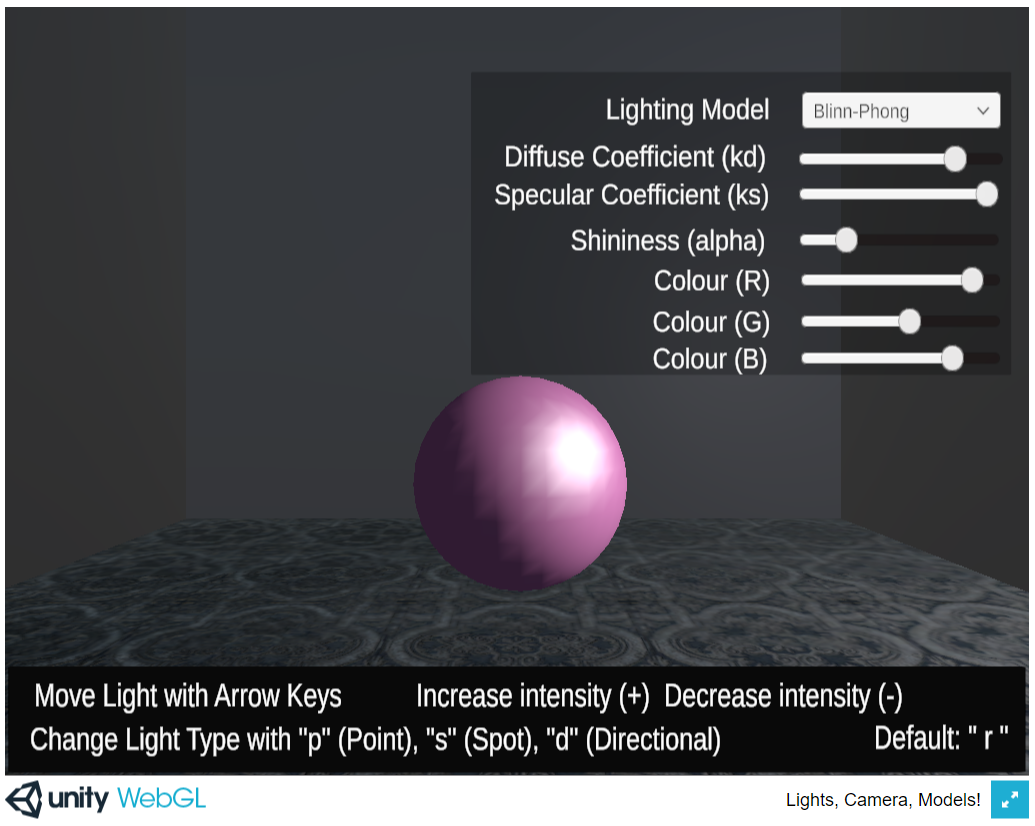
\includegraphics[scale=0.25]{./images/sphere-lit-point-moveBoundsR}
		\caption{Output Variation 2}
		\label{fig:point-bounds-right}
	\end{figure}	

	\begin{figure}[h]
		\centering
		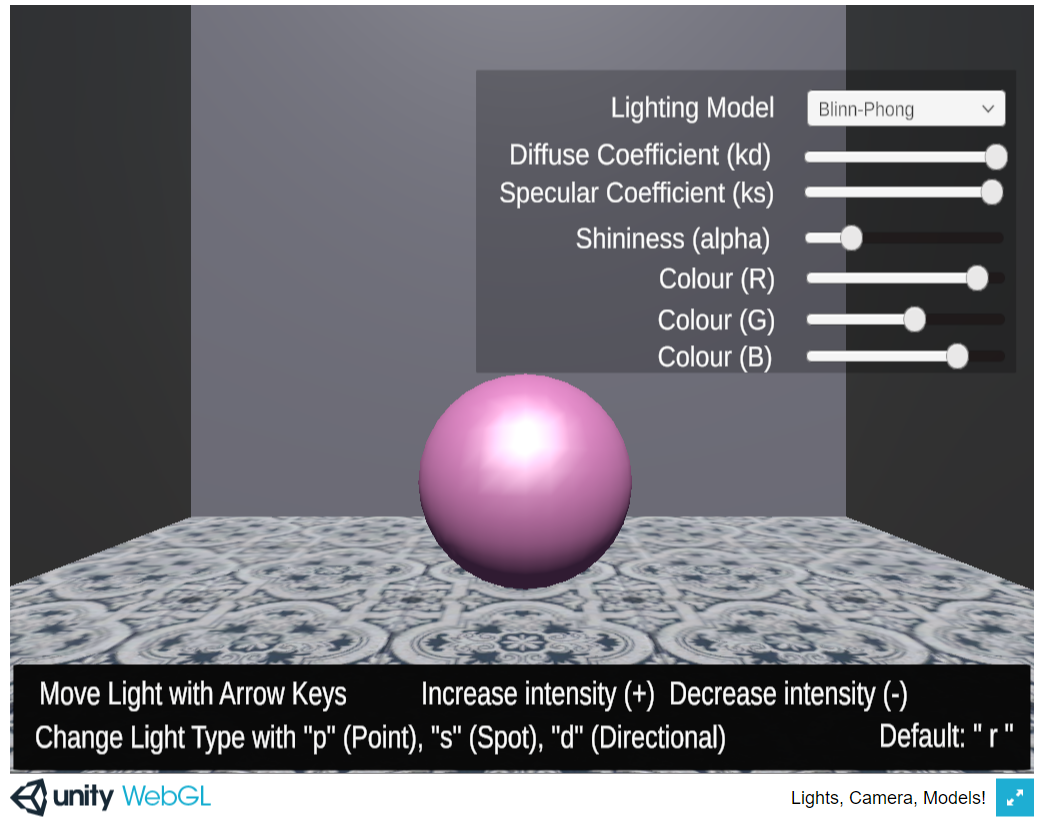
\includegraphics[scale=0.25]{./images/sphere-lit-direction}
		\caption{Output Variation 1}
		\label{fig:directional-bounds-right}
	\end{figure}

	\begin{figure}[h]
		\centering
		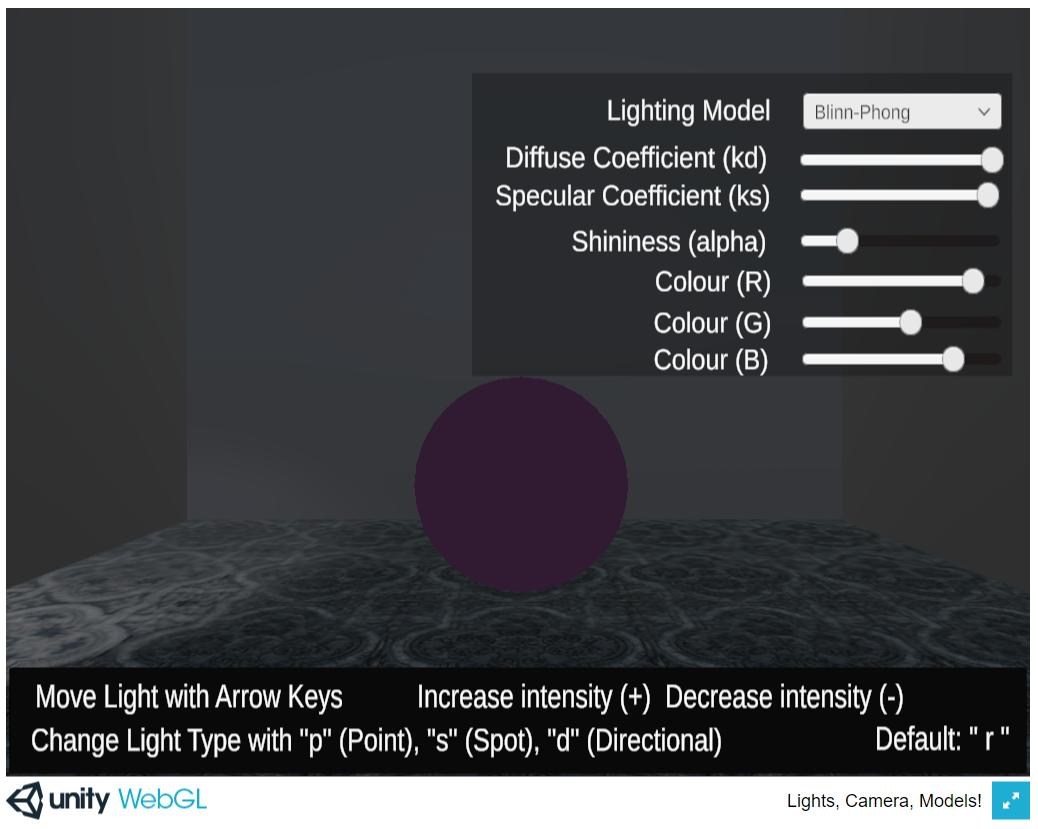
\includegraphics[scale=0.25]{./images/sphere-lit-spotlight-moveBounds}
		\caption{Output Variation 4}
		\label{fig:spotlight-bounds-left}
	\end{figure}	

	\begin{figure}[h]
		\centering
		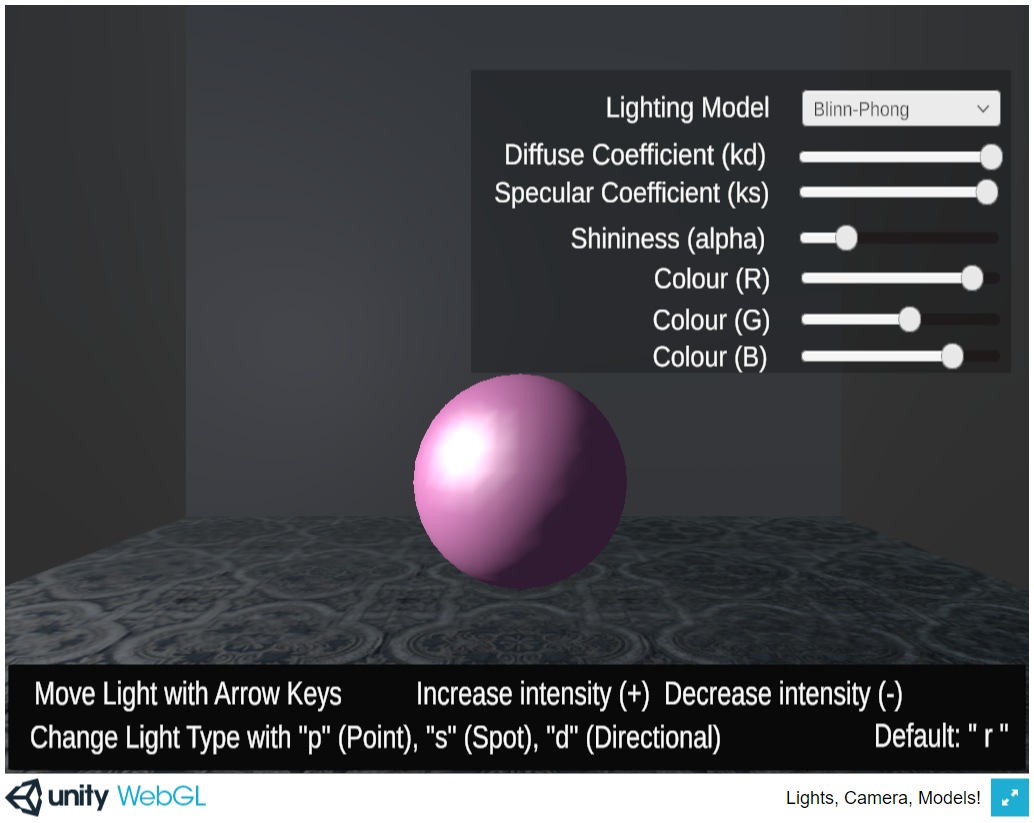
\includegraphics[scale=0.25]{./images/sphere-lit-point-moveBounds}
		\caption{Output Variation 5}
		\label{fig:point-bounds-left}
	\end{figure}	

	
	Test Case Derivation: Constraints on light position said $0 \ll 
	x \le SCENE\_HEIGHT$, which means that the centre is on the wall of the 
	scene. This means part of the light would be rendered outside the scene.
	
	How test will be performed: Valid scene is loaded. Testing framework 
	automatically assigns new position to (0,10,0). System throws an error.
	
%	\item{lightPos-valid-besideObject\\}
%	
%	Same as \textit{objPosition-valid-besideLight}. Not to be tested because it 
%	covers the same scenario.
%	
%	\item{lightPos-valid-behindObject\\}
%		
%	Same as \textit{objPosition-valid-betweenLightAndViewer}. Not to be tested 
%	because it covers the same scenario.

%%%Light Colour Change
%	\item{lightColour-valid\\}
%	
%	Control: Automatic
%	
%	Input: New (r,g,b) value for LIGHT\_COLOUR picked from GUI picker = 
%	(10,255,50).
%	
%	Output: \textit{RENDERS\_DIR/render-valid-AllInputs} with visuals changed 
%	to reflect the new light colour. All intensities need to be 
%	recalculated.
%	
%	Test Case Derivation: The intensity of the LIGHT\_COLOUR at a point is part 
%	of all lighting model calculations. Changes to the LIGHT\_COLOUR requires 
%	recalculating all of the intensity values with this new (r,g,b) information.
%	
%	How test will be performed: Valid scene is loaded. Testing framework 
%	automatically assigns new r,g,b to (10,255,50). System recalculates 
%	intensities and recolours object.		


%%Light Type Change	
	\item[\label{test:lightShape}]{lightShape-valid\\}
	
	Control: Manual
	
	Input: \\
	\textit{Variation 1}: Press s\\
	\textit{Variation 2}: Press p\\
	\textit{Variation 3}: Press d\\
	
	Output: Scene render Blinn-Phong lighting model. Intensities and incidence 
	rays are recalculated depending on the type of light source.

	\begin{figure}[h]
	\centering
	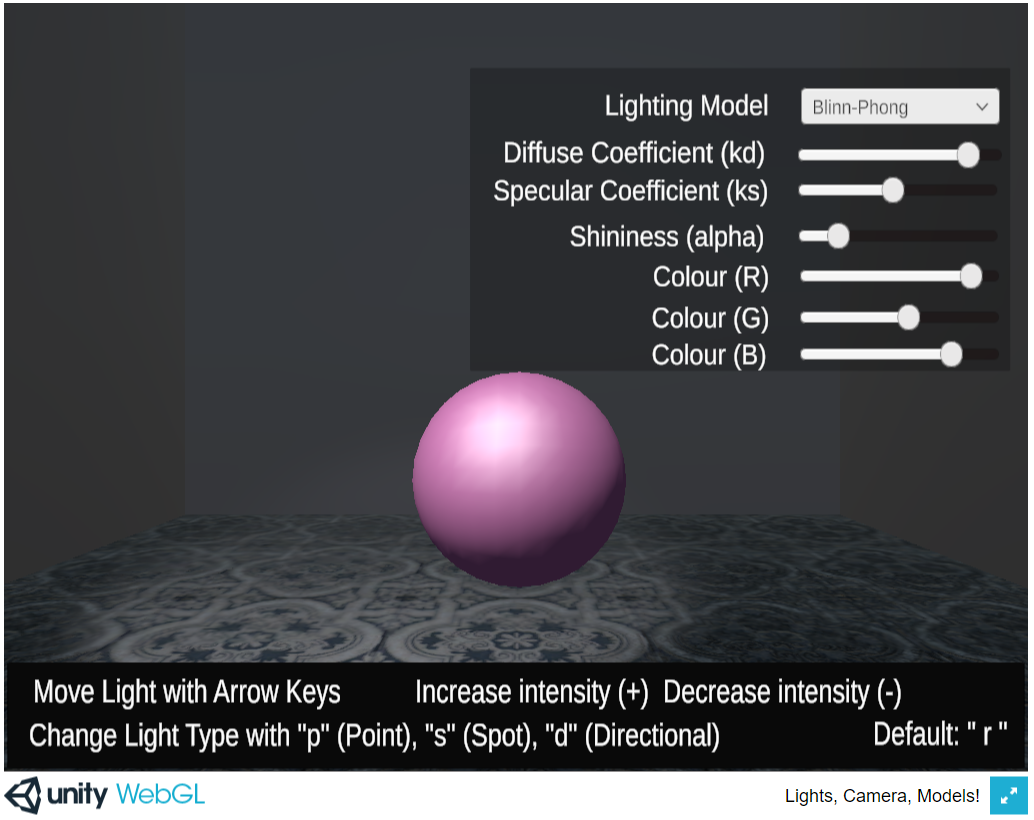
\includegraphics[scale=0.25]{./images/sphere-lit-blinnphong}
	\caption{Output Variation 1}
	\label{fig:spotlight}
	\end{figure}	
	
	\begin{figure}[h]
		\centering
		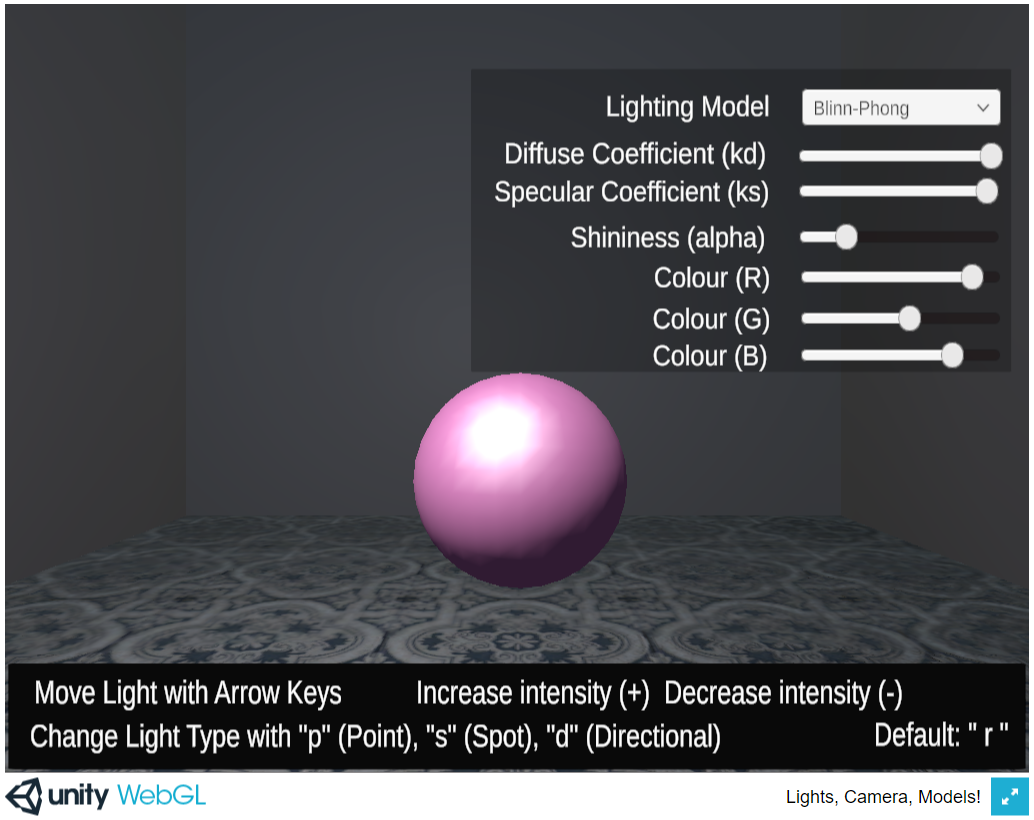
\includegraphics[scale=0.25]{./images/sphere-lit-blinnphong-point}
		\caption{Output Variation 2}
		\label{fig:point}
	\end{figure}	
	
	\begin{figure}[h]
		\centering
		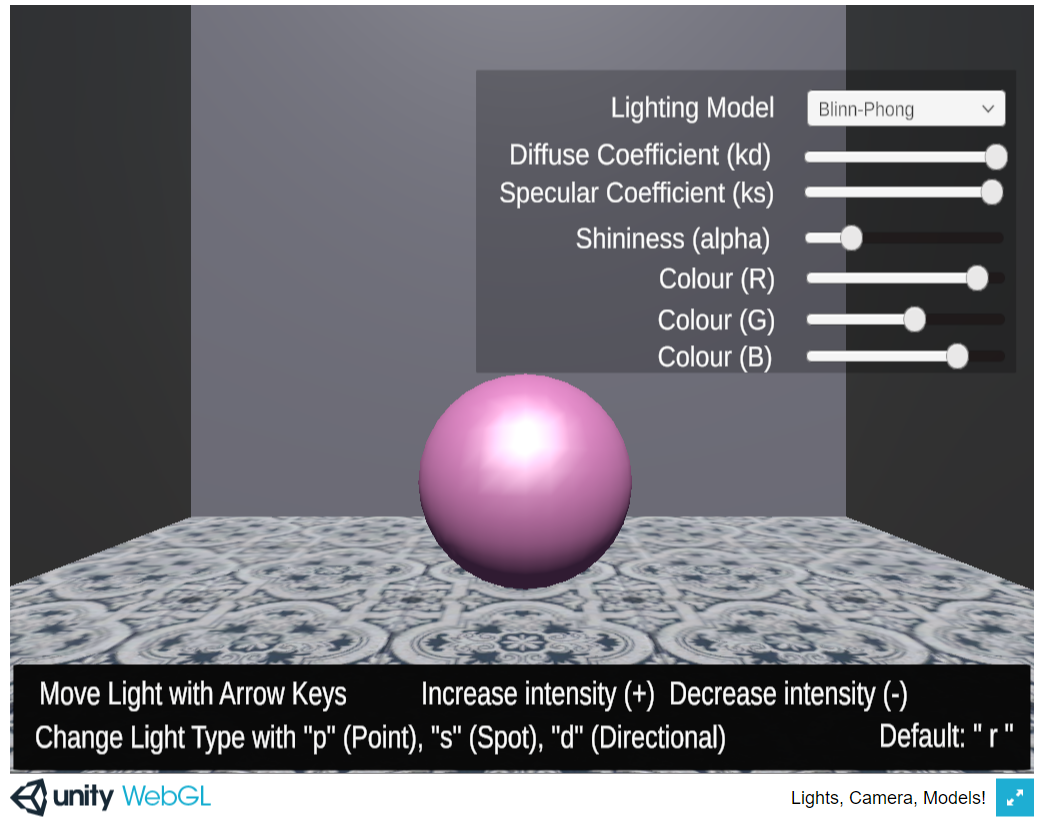
\includegraphics[scale=0.25]{./images/sphere-lit-direction}
		\caption{Output Variation 1}
		\label{fig:directional}
	\end{figure}	
	
	
	Test Case Derivation: Different types of light project light rays 
	differently. As such the system needs to adapt to the changing type of 
	lights available
	
	How test will be performed: Valid scene is loaded. Testing framework 
	automatically assigns new light type. System recalculates 
	intensities and recolours new object.
	
\end{enumerate}

\wss{There is a great variety of test cases, and many exceptions are covered,
  but I still don't see how you can tell that the scene is rendered correctly
  with respect to the mathematical model?  Do you have a pseudo-oracle that you
  can compare the results to?  Can you do a bitwise comparison between your
  image and the ``correct'' image?  If not, then you at least need some manual
  tests to verify that the scene renderings look correct.}
\sms{Due to issues with creation of the project and the way Unity works to get 
the interaction working, the majority of my tests have become System Tests that 
rely on Manual test comparing the renders for subjective same-ness.}

\subsection{Tests for Nonfunctional Requirements}
The following section outlines the test cases for the non-functional 
requirements of the system. In particular these tests focus on the usability of 
the system, encompassing aspects like ease of installation, reliability, and 
learnability.
%
%\wss{The nonfunctional requirements for accuracy will likely just reference the
%  appropriate functional tests from above.  The test cases should mention
%  reporting the relative error for these tests.}
%
%\wss{Tests related to usability could include conducting a usability test and
%  survey.}

\subsubsection{Usability}
\paragraph{Ease of Installation}
The following test cases focuses on assessing the ease of installation of the 
system. It would be unrealistic to test all potential install environments; 
however due to this being implemented in Unity, the installation environments 
of this system are limited to those that Unity can run on.

For this type of testing we are testing to pass, not testing to fail - i.e. we 
want all of these test cases to pass. We are not concerned with cases of 
invalid input, since that would just mean not installing our software. We let 
the Unity error handling inform the user if the installation is unsuccessful.

We have decided that for ease of accessibility with this software we would 
create it as a WebGL application. As the software now runs in any browser, it 
removes the need for installation tests. This section is being preserved to 
acknowledge that standalone versions would need their own testing. The specific 
installation tests have been preserved as comments.

%\begin{enumerate}
%
%\item{install-clean-modern-win\\}
%
%Type: Manual
%					
%Initial State: Clean installation of Unity version CURRENT\_VERSION on a 
%Windows 10 machine.
%					
%Input/Condition: Install system package.
%					
%Output/Result: Installation of Unity version CURRENT\_VERSION on a 
%Windows 10 machine with our system installed.
%					
%How test will be performed: The user will have a fresh install of Unity 
%CURRENT\_VERSION on a virtual windows machine. They will have a copy of the 
%system package to import into Unity. The user will then be asked to fill out 
%the Installability Evaluation borrowed from \cite{SmithEtAl2018} (See 
%\ref{tbl:installability}).
%
%\item{install-clean-modern-mac\\}
%
%Type: Manual
%
%Initial State: Clean installation of Unity version CURRENT\_VERSION on a Mac 
%OS 
%machine.
%
%Input/Condition: Install system package.
%
%Output/Result: Installation of Unity version CURRENT\_VERSION on a 
%MacOS machine with our system installed.
%
%How test will be performed: The user will have a fresh install of Unity 
%CURRENT\_VERSION on a virtual MacOS machine. They will have a copy of the 
%system package to import into Unity. The user will then be asked to fill out 
%the Installability Evaluation borrowed from \cite{SmithEtAl2018} (See 
%\ref{tbl:installability}).
%					
%\item{install-clean-previous-windows\\}
%
%Type: Manual
%
%Initial State: Clean installation of Unity version PREVIOUS\_VERSION on a 
%Windows 10 machine.
%
%Input/Condition: Install system package.
%
%Output/Result: Installation of Unity version PREVIOUS\_VERSION on a 
%Windows 10 machine with our system installed.
%
%How test will be performed: The user will have a fresh install of Unity 
%PREVIOUS\_VERSION on a virtual windows machine. They will have a copy of the 
%system package to import into Unity. The user will then be asked to fill out 
%the Installability Evaluation borrowed from \cite{SmithEtAl2018} (See 
%\ref{tbl:installability}).
%
%\item{install-clean-previous-mac\\}
%
%Type: Manual
%
%Initial State: Clean installation of Unity version PREVIOUS\_VERSION on a Mac 
%OS machine.
%
%Input/Condition: Install system package.
%
%Output/Result: Installation of Unity version PREVIOUS\_VERSION on a 
%MacOS machine with our system installed.
%
%How test will be performed: The user will have a fresh install of Unity 
%PREVIOUS\_VERSION on a virtual MacOS machine. They will have a copy of the 
%system package to import into Unity. The user will then be asked to fill out 
%the Installability Evaluation borrowed from \cite{SmithEtAl2018} (See 
%\ref{tbl:installability}).
%
%\end{enumerate}

%\subsubsection{Reliability}
%The following test cases focus on assessing the reliability of the system to 
%repeatedly perform routine tasks. The purpose of these tests is to determine 
%the load the system, and ensure that the output is reliable. These tests run 
%the system through the functional test cases multiple times in succession.
%
%\begin{enumerate}
%	
%	\item{reliable-loading\\}
%	
%	Type: Automatic \wss{How is this automated?  Do you have a unit testing
%          framework that can do this?}
%	
%	Initial State: No scene loaded.
%	
%	Input/Condition: \textit{SCENE\_DIR/valid-AllInputs.JSON}(See 
%	\ref{in:valid-All})
%	
%	Output/Result: \textit{SCENE\_DIR/valid-AllInputs.JSON}
%	
%	How test will be performed: The system shall perform test 
%	\textit{loadScene-allValid} RELIABILITY\_THRESHOLD times in succession. The 
%	output should be the same as doing it once.
%
%\wss{Interesting test case.  It does sometimes confuse systems to do something
%  like this twice.  Good idea.}
%
%	\item{reliable-taskSwitch\\}
%	
%	Type: Automatic
%	
%	Initial State: No scene loaded.
%	
%	Input/Condition: \textit{SCENE\_DIR/valid-AllInputs.JSON}(See 
%	\ref{in:valid-All}), $k_{a} = 0.5$, 
%	$k_{d} = 0.5$, $k_{s} = 0.8$, $\alpha = 10$
%	
%	Output/Result: \textit{SCENE\_DIR/valid-AllInputs.JSON}
%	
%	How test will be performed: The system shall perform test 
%	\textit{loadScene-allValid} and then in sequence make changes to the object 
%	properties. The output file should have the following values:
%
%\end{enumerate}

\subsubsection{Learnability}
The following test cases focus on understanding how easy the system is to learn 
for new users. In this case, we consider new users as those who are have less 
than 1 years experience in working with 3D graphics and lighting (i.e. Unity, 
or equivalent). The purpose of these tests is to see if a user with no 
background knowledge of these types of systems can perform basic operations 
successfully with no assistance.

The rationale is to see learnability as a ratio of mistakes made to task 
completion time. Mistakes in this case constitute errors and the amount of 
times they asked for assistance or sought ought documentation. The reason these 
are captured in mistakes is because our software ought to be intuitive to use; 
any time the user requires assistance it is because our software was 
unintuitive.

All learnability test cases share the following properties:
\begin{itemize}
	\item[] Initial State: No scene loaded.
\end{itemize}
\begin{enumerate}
	
	\item{learnability-loadScene\\}
	
	Type: Manual
	
	Input/Condition: \textit{SCENE\_DIR/valid-AllInputs.JSON}(See 
	\ref{in:valid-All})
	
	Output/Result: \textit{SCENE\_DIR/valid-AllInputs.JSON}. Time to 
	completion. Number of errors. Number of times they sought assistance.
	
	How test will be performed: The user will have Unity open with the system 
	installed. The user will proceed to load the input file to the system. Time 
	will be measured from when the user opens Unity to when the output file is 
	rendered. The number of errors will be measured as the number of misclicks 
	made while performing this task. The number of times they sought assistance 
	will me measured as times when they asked for help, or consulted any 
	documentation. Users will also fill out the (\ref{survey:novice}) or 
	Expert (\ref{survey:expert}) Usability 
	Survey depending on their familiarity with other 3D graphics programs.

	\item{learnability-taskSequence\\}
	
	Type: Manual
	
	Input/Condition: \textit{SCENE\_DIR/valid-AllInputs.JSON}(See 
	\ref{in:valid-All}), $k_{a} = 0.5$, 
	$k_{d} = 0.5$, $k_{s} = 0.8$, $\alpha = 10$.
	
	Output/Result: \textit{SCENE\_DIR/valid-AllInputs.JSON}. Time to 
	completion. Number of errors. Number of times they sought assistance.
	
	How test will be performed: The user will have Unity open with the system 
	installed. The user will proceed to load the input file to the system. The 
	user will proceed to change the values of the object material properties to 
	those given in the input. Time will be measured from when the user opens 
	Unity to when the output file is rendered. The number of errors will be 
	measured as the number of misclicks/mistypes made while performing this 
	task. The number of times they sought assistance 
	will me measured as times when they asked for help, or consulted any 
	documentation. Users will also fill out the Novice (\ref{survey:novice}) or 
	Expert (\ref{survey:expert}) Usability Survey depending on their 
	familiarity with other 3D graphics programs.

\end{enumerate}

\wss{The learnability measurements sound good to me.  I hope you have time to at
least do a few measurements.}

\subsection{Traceability Between Test Cases and Requirements}
The following section summarizes the relationships between test cases and 
requirements. We have restated the requirements originally laid out in  the CA 
here for convenience. Note that requirements 12-14 are not covered by test 
cases - this is because their requirements are not part of the objective of 
this test plan.

\paragraph{Requirements from CA} \wss{For maintainability reasons, it usually
  isn't a good idea to copy and paste between documents.  A cross-reference to
  the CA document should be all that you need.}
~\newline
\noindent 
\begin{itemize}
	%%Reliability
	\item[R\refstepcounter{reqnum}\thereqnum \label{R_Inputs1}:] When presented 
	with a scene in a file, the system shall correctly read from file the 
	input data for light source(s) and object(s).
	%%Rationale: The system may be provided a file with scene data. I want to 
	%%leave this open that there could be a GUI with dropdown selections to 
	%%make this process easier - ergo the "when".
	
	\item[R\refstepcounter{reqnum}\thereqnum \label{R_Inputs1Err}:]System 
	responds with specific error message when system cannot read input files.
	
	\item[R\refstepcounter{reqnum}\thereqnum \label{R_Inputs1Err-Def}:]	The 
	system asks user if they would like to use the default settings when scene 
	size, shading model, and/or reflection model information is missing from 
	input, and applies (DEF\_HEIGHT, DEF\_WIDTH, DEF\_DEPTH), DEF\_SHADE and/or 
	DEF\_LIGHT if the user answers yes.
	%%Rationale: The system should be robust enough to render a scene when 
	%%given just the light source, object information. This gives new users 
	%%room to learn the input method. 
	
	\item[R\refstepcounter{reqnum}\thereqnum \label{R_DefaultScene}:]When no 
	input file is given, the system provides a default scene of dimension 
	(DEF\_HEIGHT, DEF\_WIDTH, DEF\_DEPTH) with one point light source with the 
	default light colour, one sphere with the default material properties, 
	rendered using default shading (DEF\_SHADE) and lighting (DEF\_LIGHT).
	%%Rationale: The system needs a default test case that shows minimum 
	%%functioning.
	
	\item[R\refstepcounter{reqnum}\thereqnum \label{R_Inputs2}:]The system 
	shall verify that all input data meets constraints laid out in the CA.
	
	\item[R\refstepcounter{reqnum}\thereqnum \label{R_Inputs2Err}:] The system 
	responds with specific error message when user inputs contain errors (type 
	mismatch, data outside of constraints).
	
	\item[R\refstepcounter{reqnum}\thereqnum \label{R_Calculate1}:] The library 
	shall correctly calculate the surface normals for object(s) based on 
	shading model.
	
	\item[R\refstepcounter{reqnum}\thereqnum \label{R_Calculate2}:] The library 
	shall calculate the incidence and reflection vectors off of object(s) 
	surface(s) based on light position(s), object(s) properties, shading model 
	and observer position.
	
	\item[R\refstepcounter{reqnum}\thereqnum \label{R_Calculate3}:] The library 
	shall calculate the light intensity based on light position(s), object(s) 
	material properties, and shading model.
	
	\item[R\refstepcounter{reqnum}\thereqnum \label{R_Calculate4}:] The library 
	shall calculate the final colour object(s) faces based on the intensities 
	calculated in \rref{R_Calculate3}.
	
	\item[R\refstepcounter{reqnum}\thereqnum \label{R_Output}:] The library 
	will output code for a lit and shaded scene.
	
	\item[R\refstepcounter{reqnum}\thereqnum \label{R_Performance}:]Users can 
	render a default scene (define in \rref{R_DefaultScene}) faster than in 
	OpenGL.
	%%Rationale: Performance comparison against main competitor.
%% Productivity Requirements
	\item[R\refstepcounter{reqnum}\thereqnum 
	\label{NFR-Productivity-InputMods}:] 
	The addition of new input methods should not affect the usability of the 
	system.
	%%Rationale: The input methods should be a secret of the system that 
	%%doesn't affect the interface. I'm not sure where to capture this. 
	\item[R\refstepcounter{reqnum}\thereqnum 
	\label{NFR-Productivity-Modifications}:] 
	The addition of new lighting models, shading models, types of light sources 
	and/or types of objects should be completable in 
	MODIFICATION\_TIME\_THRESHOLD.
	%%Rationale: The system should allow for expansion with new approximations; 
	%%the design of the system should allow for new models or types to be 
	%%inserted with minimal effort since all should require the same underlying 
	%%information (object material properties, luminous intensity, etc.) The 
	%%ability to modify the system in a defined amount of time adds to the 
	%%overall productivity of the software as people would be able to expand 
	%%and use it in a minimal amount of time. 
	%% Usability Requirements	
	\item[R\refstepcounter{reqnum}\thereqnum \label{NFR-Usability-Install}:] 
	USABILITY\_THRESHOLD \% of users can install the system without requiring 
	assistance.
	%%Rationale: System usability is directly affected by whether it is easy to 
	%%install.
	\item[R\refstepcounter{reqnum}\thereqnum \label{NFR-Usability-load}:] 
	USABILITY\_THRESHOLD \% of users can load an existing scene with no 
	assistance.
	%%Rationale: Usability is determined by ability to perform the basic 
	%%functions without needing assistance/making errors. It's unreasonable at 
	%%this stage to dictate the number of errors that is a threshold since I 
	%%haven't figured out what the system interface is going to look like - so 
	%%the best method of judging at the moment is whether they can perform the 
	%%tasks with no assistance regardless of how long it takes. Future 
	%%refinements of this should indicate how many steps this particular 
	%%interaction should be to quantify this data.
	\item[R\refstepcounter{reqnum}\thereqnum \label{NFR-Usability-changes}:] 
	USABILITY\_THRESHOLD \% of users can change the parameters of the lighting 
	models and re-render an existing scene with no assistance.
	%%Rationale: same as above. The ability to perform this also informs us 
	%%about the user's ability to recover from errors. If they entered the 
	%%wrong model for example, they can enact this ability to correct it.
	\item[R\refstepcounter{reqnum}\thereqnum \label{NFR-Usability-new}:] 
	USABILITY\_THRESHOLD \% of users can initialise a new scene with the 
	default parameters (default object, light source, lighting model, and 
	shader) with no assistance.
	%%Rationale: same as above.		
	\item[R\refstepcounter{reqnum}\thereqnum \label{NFR-Usability-perceived}:] 
	USABILITY\_THRESHOLD \% of users perceive \famname to be easier to use than 
	OpenGL.
	%%Rationale: Way to qualitatively quantify how this system compares to on 
	%%of its competitors.		
	\item[R\refstepcounter{reqnum}\thereqnum 
	\label{NFR-Usability-control-perceived}:] 
	USABILITY\_THRESHOLD \% of users perceive \famname to allow them more 
	control than the built in Unity shader options.
	%%Rationale: Way to qualitatively quantify how this system compares to on 
	%%of its competitors.	
\end{itemize}

%\wss{Provide a table that shows which test cases are supporting which
%  requirements.}

%\begin{landscape}
	\begin{tabular}{|p{5cm}|l|l|l|l|l|l|l|l|l|l|l|}
		\hline
		& \multicolumn{11}{c}{Functional Requirements}\\
		\hline
		\textbf{Test Case} & \textbf{R1} & \textbf{R2} & \textbf{R3} & 
		\textbf{R4} & \textbf{R5} & \textbf{R6} & \textbf{R7} & \textbf{R8} & 
		\textbf{R9} & \textbf{R10} & \textbf{R11} \\
		\hline
		loadScene-allValid & X & & & & X &  & X & X & X & X & X \\
		loadScene-validMissingSome & X &  & X &  & X & & X & X & X & X & X\\
		loadScene-fileExistNoData & X &  &  & X & X & & X & X & X	& X & X\\
		loadScene-invalidInput &  & X &  & & X & X & & & & & \\
		createDefault-validMissingData & & & X & & & & X &X& X & X & X\\
		createDefault-fileExistNoData & & & & X & & & X & X &X & X & X\\
		lightModel-valid & X & & & & X & & & & X & X & X\\
		shadingModel-valid & X & & & & X & & X & & X & X &X 
		\\				 				
		objMaterialPropChange-valid-ks & & & & & X & & & & X & X & X\\
		objMaterialPropChange-valid-kd & & & & & X & & & & X & X & X\\
		objMaterialPropChange-valid-ka & & & & & X & & & & X & X & X\\
		objMaterialPropChange-valid-$\alpha$ & & & & & X & & & & X & X & X\\
		objMaterialPropChange-invalid-ks & & & & & X &X & & & X & X & X\\
		objMaterialPropChange-invalid-kd & & & & & X &X & & & X & X & X\\
		objMaterialPropChange-invalid-ka & & & & & X &X & & & X & X & X\\
		objMaterialPropChange-invalid-$\alpha$ & & & & & X &X & & & X & X & X\\
		\hline
	\end{tabular}
%\end{landscape}
~\newline
\begin{tabular}{|p{5cm}|l|l|l|l|l|l|l|l|l|l|l}
	\hline
	& \multicolumn{11}{c}{Functional Requirements}\\
	\hline
	\textbf{Test Case} & \textbf{R1} & \textbf{R2} & \textbf{R3} & \textbf{R4} 
	& \textbf{R5} & \textbf{R6} & \textbf{R7} & \textbf{R8} & \textbf{R9} & 
	\textbf{R10} & \textbf{R11} \\
	\hline
	objMaterialPropChange-bound-ks & & & & & X & & & & X & X & X\\
	objMaterialPropChange-bound-kd & & & & & X & & & & X & X & X\\
	objMaterialPropChange-bound-ka & & & & & X & & & & X & X & X\\
	objMaterialPropChange-bound-$\alpha$ & & & & & X & & & & X & X & X\\
	objPosition-valid & & & & & X & & X	& X & X & X & X\\	
	objPosition-invalid-outBounds & & & & & X & X & X	& X & X & X & X\\
	objPosition-invalid-onLight & & & & & X & X & X	& X & X & X & X\\			
	objPosition-invalid-onObserver & & & & & X & X & X	& X & X & X & 
	X\\			
	objPosition-valid-edgeOfRoom & & & & & X & & X	& X & X & X & X\\
	objPosition-valid-betweenLightAndViewer & & & & & X & & X	& X & X & X & 
	X\\
	objPosition-valid-besideLight & & & & & X & & X	& X & X & X & X\\
	objColour-valid-base & & & & & X & & & & X & X & X\\	
	objColour-valid-specular & & & & & X & & & & X & X & X\\					
	objShape-valid & & & & & X & & & & X & X & X\\			
	lightPos-valid & & & & & X & & X & X & X & X & X\\	
	lightPos-invalid-outBounds & & & & & X & X & X	& X & X & X & X\\
	lightPos-invalid-onObj & & & & & X & X & X	& X & X & X & X\\			
	lightPos-invalid-onObserver & & & & & X & X & X	& X & X & X & X\\
	lightPos-valid-boundary & & & & & X & & X & X & X & X & X\\
	objPosition-valid-behindObject & & & & & X & & X & X & X & X & X\\
	objPosition-valid-besideObject & & & & & X & & X & X & X & X & X\\
	lightColour-valid & & & & & X & & X & X & X & X & X\\					
	lightShape-valid & & & & & X & & X & X & X & X & 
	X\\
	\hline									
\end{tabular}

%\begin{landscape}
	\begin{tabular}{|p{5cm}|l|l|l|l|l|l|l|l|l|}
		\hline
		& \multicolumn{9}{c}{Non-Functional Requirements}\\
		\textbf{Test Case} & \textbf{R12} & \textbf{R13} & \textbf{R14} & 
		\textbf{R15} & \textbf{R16} & \textbf{R17} & \textbf{R18} & 
		\textbf{R19} & 
		\textbf{R20} \\
		\hline
		loadScene-validMissingSome & & & & & & & X & & \\
		loadScene-fileExistNoData & & & & & & & X & & \\
		install-clean-modern-win & & & & X & & & &  & \\
		install-clean-modern-mac & & & & X & & & &  & \\
		install-clean-previous-win & & & & X & & & &  & \\
		install-clean-previous-mac & & & & X & & & &  & \\
		reliable-loading & & & & & X & & & & \\
		reliable-taskSwitch & & & & & X & X & & & \\
		learnability-loadScene & & & & & X & & & X & X \\
		learnability-taskSequence & & & & & X & X & & X & 
		X\\				 				
		\hline		
	\end{tabular}
%\end{landscape}
				
\bibliographystyle {plainnat}
\bibliography {../../refs/References}

\newpage

%\section{Appendix}
%\subsection{Input Files}
%This section contains the contents of the input files used for the test cases.
%
%\paragraph{valid-AllInputs.json}\label{in:valid-All}
%~\newline
%\begin{lstlisting}
%{
%	"Height" : 50,
%	"Width" : 50,
%	"Depth" : 50,
%
%	"Object":[
%		{
%			"type": "sphere",
%			"position": [10,0,10],
%			"size": 1,
%			"ka": 1,
%			"kd": 1,
%			"ks": 0.5,
%			"alpha": 1,
%			"base_colour": [35,74,35],
%			"spec_colour": [255,255,255],			
%		}
%	],
%	
%	"LightSource": [
%		{
%			"type": "point",
%			"position": [5,10,0],
%			"light_colour": [255,255,255],
%			"intensity": [10,10,10],
%		}
%	],
%	
%	"Observer" : [
%		{
%			"position" : [0,0,0],
%			"direction" : [1,0,1]
%		}
%	],
%	
%	"ShadingModel" : "Gouraud",
%	"LightingModel" : "Phong"
%}
%\end{lstlisting}
%
%\paragraph{valid-MissingData.json}\label{in:valid-Miss}
%~\newline
%\begin{lstlisting}
%{
%	"Height" : 50,
%	"Width" : 50,
%	"Depth" : 50,
%	
%	"Object":[
%		{
%			"type": "sphere",
%			"position": [10,0,10],
%			"size": 1,
%			"ka": 1,
%			"kd": 1,
%			"ks": 0.5,
%			"alpha": 1,
%			"base_colour": [35,74,35],
%			"spec_colour": [255,255,255],			
%		}
%	],
%	
%	"LightSource": [
%		{
%			"type": "point",
%			"position": [5,10,0],
%			"light_colour": [255,255,255],
%			"intensity": [10,10,10],
%		}
%	],
%	
%	"Observer" : [
%		{
%			"position" : [0,0,0],
%			"direction" : [1,0,1]
%		}
%	],
%	
%	"ShadingModel" : ,
%	"LightingModel" : 
%}
%\end{lstlisting}
%
%\paragraph{valid-NoData.json}\label{in:valid-No}
%~\newline
%\begin{lstlisting}
%{
%
%}
%\end{lstlisting}
%
%\paragraph{valid-invalid.json}\label{in:invalid}
%~\newline
%\begin{lstlisting}
%{
%	"Height" : 50,
%	"Width" : 50,
%	"Depth" : 50,
%	
%	"Object":[
%		{
%			"type": "sphere",
%			"position": [10,0,10],
%			"size": 1,
%			"ka": 2,
%			"kd": 1,
%			"ks": 0.5,
%			"alpha": 1,
%			"base_colour": [35,74,35],
%			"spec_colour": [255,255,255],			
%		}
%	],
%	
%	"LightSource": [
%		{
%			"type": "point",
%			"position": [5,10,0],
%			"light_colour": [255,255,255],
%			"intensity": [10,10,10],
%		}
%	],
%	
%	"Observer" : [
%		{
%			"position" : [0,0,0],
%			"direction" : [1,0,1]
%		}
%	],
%	
%	"ShadingModel" : "Flat",
%	"LightingModel" : "Lambertian" 
%}
%\end{lstlisting}
%
%\subsection{Installability Evaluation \protect
%	\cite{SmithEtAl2018}}
%\begin{table}[h]
%	\begin{tabular}{p{10cm}p{5cm}}
%		\hline
%		\multicolumn{2}{l}{\textbf{Installability}(Measured via installation on 
%		a virtual machine.)} \\
%		\hline
%		Are there installation instructions? & ({yes, no}) \\
%		Are the installation instructions linear? & ({yes, no, n/a}) \\
%		Is there something in place to automate the installation? & ({yes, no}) 
%		\\		
%		Is there a specified way to validate the installation, such as a test 
%		suite? & ({yes, no}) \\
%		How many steps were involved in the installation? & (number) \\
%		How many software packages need to be installed before or during 
%		installation? & (number) \\
%		(I) Run uninstall, if available. Were any obvious problems caused? & 
%		({unavail, yes, no}) \\
%		Overall impression? & ({1...10}) \\
%		\hline
%	\end{tabular}
%	\caption{Installability Evaluation from \protect\cite{SmithEtAl2018}}
%	\label{tbl:installability}
%\end{table}

\subsection{Symbolic Parameters}
The definition of the test cases will call for SYMBOLIC\_CONSTANTS.
Their values are defined in this section for easy maintenance.

\begin{tabular}{p{10cm}|p{5cm}}
	\textbf{Symbolic Constant} & \textbf{Value} \\
	\hline
	DEF\_HEIGHT & 10 \\
	DEF\_WIDTH & 10 \\
	DEF\_DEPTH & 10 \\
	DEF\_SHADE & Gouraud \\
	DEF\_LIGHT & Lambertian \\
	PREVIOUS\_VERSION & 2018.2.16 \\
	CURRENT\_VERSION & 2019.2.11\\
	RELIABILITY\_THRESHOLD & 90\%\\
	USABILITY\_THRESHOLD & 90\%\\
	MODIFICATION\_TIME\_THRESHOLD & 2 DAYS \\
\end{tabular}

\subsection{Usability Survey Questions?}
The following section outlines usability surveys for the system. It is split up 
into two surveys: for novices, and for experts. The rationale for splitting the 
survey up is because of the different expectations each user group will have 
for the software. Novice users tend to focus on completing the task, and the 
learnability of the software. Expert users tend to focus on task efficiency, 
and the extendability of the software.

\paragraph{Novice User Usability Survey}\label{survey:novice}
~\newline
\begin{tabular}{p{8cm}|p{8cm}}
	\hline
	\textbf{Question} & \textbf{Rationale} \\
	\hline
	%%Installation
	On a scale of 1 (extremely difficult) to 5 (extremely easy), how easy was 
	the installation of the system into Unity? & To measure the perceived ease 
	of installation; the installability evaluation grades the ease of 
	installation documentation and process (through number of steps) without 
	accounting for the user base's existing experience with installing 
	software. For example, an installation with 5 large steps may be more 
	difficult to follow than one with 10 small steps. The installation process 
	should be intuitive enough that the user doesn't need documentation.\\
	%%Learning/Retention
	On a scale of 1 (not at all confident) to 5 (extremely confident), how 
	confident are you that you could load a scene in this system? & To quantify 
	learnability (and retention) of basic function --- loading a scene. \\
	On a scale of 1 (not at all confident) to 5 (extremely confident), how 
	confident are you that you could change the material parameters of an 
	object in this system? & To quantify learnability (and retention) of basic 
	function --- modifying an object's properties. \\
	On a scale of 1 (not at all confident) to 5 (extremely confident), how 
	confident are you that you could change the position of an object in this 
	system? & To quantify learnability (and retention) of basic function --- 
	modifying an object's position. \\	
	On a scale of 1 (not at all confident) to 5 (extremely confident), how 
	confident are you that you could change the parameters of light source in 
	this system? & To quantify learnability (and retention) of basic function 
	--- modifying a light source. \\	
	On a scale of 1 (not at all confident) to 5 (extremely confident), how 
	confident are you that the system will output a correctly rendered scene? & 
	To quantify trust between the user and the system --- effectively measuring 
	the perceived reliability. \\
	%%Would they use		
	On a scale of 1 (extremely unlikely) to 5 (extremely likely), how 
	likely are you to use this system for local illumination? & To judge 
	whether the system perceivably satisfies their needs. \\
	\hline
\end{tabular}

\paragraph{Expert User Usability Survey}\label{survey:expert}
~\newline
\begin{tabular}{p{8cm}|p{8cm}}
	\hline
	\textbf{Question} & \textbf{Rationale} \\
	\hline
%%Installation
	On a scale of 1 (extremely difficult) to 5 (extremely easy), how easy was 
	the installation of the system into Unity? & To measure the perceived ease 
	of installation; the installability evaluation grades the ease of 
	installation documentation and process (through number of steps) without 
	accounting for the user base's existing experience with installing 
	software. For example, an installation with 5 large steps may be more 
	difficult to follow than one with 10 small steps. The installation process 
	should be intuitive enough that the user doesn't need documentation.\\
%%Learning/Retention
	On a scale of 1 (not at all confident) to 5 (extremely confident), how 
	confident are you that you could load a scene in this system? & To quantify 
	learnability (and retention) of basic function --- loading a scene. \\
	On a scale of 1 (not at all confident) to 5 (extremely confident), how 
	confident are you that you could change the material parameters of an 
	object in this system? & To quantify learnability (and retention) of basic 
	function --- modifying an object's properties. \\
	On a scale of 1 (not at all confident) to 5 (extremely confident), how 
	confident are you that you could change the position of an object in this 
	system? & To quantify learnability (and retention) of basic function --- 
	modifying an object's position. \\	
	On a scale of 1 (not at all confident) to 5 (extremely confident), how 
	confident are you that you could change the parameters of light source in 
	this system? & To quantify learnability (and retention) of basic function 
	--- modifying a light source. \\	
	On a scale of 1 (not at all confident) to 5 (extremely confident), how 
	confident are you that the system will output a correctly rendered scene? & 
	To quantify trust between the user and the system --- effectively measuring 
	the perceived reliability. \\
%%Comparison to other systems used
	Which system was easiest to use for loading a scene (circle one): Unity, 
	System, OpenGL & The point is to have them single out preferences against 
	the competition for this specific task.\\
	Which system was easiest to use for changing the properties of an object 
	(circle one): Unity, System, OpenGL & The point is to have them single out 
	preferences against the competition for this specific task.\\	
	Which system was easiest to use for changing the properties of light source 
	(circle one): Unity, System, OpenGL & The point is to have them single out 
	preferences against the competition for this specific task.\\		
	\hline
\end{tabular}

~\newline
\paragraph{Expert User Usability Survey (continued)}
~\newline
\begin{tabular}{p{8cm}|p{8cm}}
	\hline
	\textbf{Question} & \textbf{Rationale} \\
	\hline
%%Comparison to other system continued
	Which system was easiest to create a scene for (circle one): Unity, System, 
	OpenGL & The point is to have them single out preferences against the 
	competition for this specific task.\\	
	%%Extensibility of Features
	Which system handles the most lighting options (circle one): OpenGL, Unity, 
	System. & The showcase which system is considered the most extendable. \\
	%%Would they use		
	On a scale of 1 (extremely unlikely) to 5 (extremely likely), how 
	likely are you to use this system for local illumination? & To judge 
	whether the system perceivably satisfies their needs. \\
	\hline
\end{tabular}

%\wss{This is a section that would be appropriate for some projects.}

\end{document}